\documentclass{article} % For LaTeX2e
\usepackage{iclr2026_conference,times}
\usepackage{enumitem}
\usepackage{graphicx}
% mini model icon; tweak height to taste
\newcommand{\micon}[1]{%
  \raisebox{-0.25\height}{\includegraphics[height=1em]{icons/#1}}}
\usepackage{amsmath}
\usepackage{tikz}
\usetikzlibrary{shapes.geometric}
\usetikzlibrary{arrows.meta, positioning}
\usepackage{hyperref}
\usepackage{url}
\usepackage{booktabs}
\usepackage{multirow}
\usepackage[compatibility=false]{caption}
\usepackage{subcaption} % Added to define the subfigure environment
\usepackage{amsfonts}

\usetikzlibrary{backgrounds}


\usepackage{wrapfig}
\usetikzlibrary{arrows.meta,positioning}
\usepackage[percent]{overpic}   % <- needed for the (b)/(c) panel tags
% mini model icon; tweak height to taste
\renewcommand{\micon}[1]{%
  \raisebox{-0.25\height}{\includegraphics[height=1em]{icons/#1}}}

\usepackage[table]{xcolor}
\title{Forecasting as Inductive World Modeling}

% For an anonymous ICLR submission, remove the author block below or keep
% \iclrfinalcopy commented out as required by the venue's submission rules.
\author{
Liv d'Aliberti \\
Department of Computer Science \\
Princeton University \\
\texttt{od2961@princeton.edu}
\And
Lillio Mok \\
Toyota Research Institute \\
\And
Kate Sieck \\
Toyota Research Institute \\
\And
Manoel Horta Ribeiro \\
Department of Computer Science \\
Princeton University \\
\texttt{manoel@cs.princeton.edu}
}

% \iclrfinalcopy % Uncomment for camera-ready version, but NOT for anonymous submission.
\begin{document}

\maketitle


\begin{abstract}
Judgmental forecasting is a natural but incomplete diagnostic for whether language agents construct inductive world models.
Accurate forecasts may reflect coherent, updateable event models, but they may also arise from recalling similar cases, imitating crowds, or rationalizing after the fact.
We test whether agents go beyond these shortcuts across two settings.
First, on unresolved prediction-market questions, frontier agents update coherently and selectively, revising far more on causally relevant evidence than on irrelevant evidence.
Second, in a simulated task with known latent structure, a revealing contrast emerges: the strongest agents leverage useful priors to estimate the hidden factor from few observations, when a matched statistical forecaster cannot, but once enough data accumulates, the statistical forecaster overtakes the agent.
This early-data regime matters because real forecasting often affords sparse evidence and a single attempt. Finally, forecasting training improves this ability and generalizes to held-out synthetic worlds and real forecasting questions.
Together, these results show that language agents learn inductive world models that support coherent updating, sparse-evidence inference, and transfer beyond the training distribution.
\end{abstract}

\section{Introduction}
\begin{wrapfigure}{r}{0.5\textwidth}
\vspace{-2.0em}
\centering
\includegraphics[width=0.48\textwidth]{iclr2026/figures/teaser.drawio.pdf}
\vspace{-0.5cm}
\caption{
\small
After observing two heads in a row at a carnival coin-flipping game, forecasts differ depending on whether the coin is treated as fair, streaky, or rigged. Frontier LLMs, Claude Opus-4.8, DS-V4-Pro, and GPT-5.4, asked to carry out a judgmental forecasting, appear to use  an inductive world model.}
\vspace{-0.5cm}
\label{fig:world-knowledge-evidence}
\end{wrapfigure}

Judgmental forecasting is a demanding form of reasoning central to decisions about political, social, and economic futures.
Unlike settings with abundant historical data for statistical extrapolation, judgmental forecasting requires integrating sparse, noisy evidence with contextual knowledge to form calibrated beliefs about future outcomes~\citep{tetlock2016superforecasting,mellers2014psychological,lawrence2006judgmental}. We argue this makes \textbf{judgmental forecasting a natural setting for studying inductive world modeling}, i.e., the ability to infer latent states, mechanisms, and dynamics from limited observations, and to use those inferred structures to predict how the world may evolve~\citep{tenenbaum2006theory,griffiths2010probabilistic,tenenbaum2011mind,lake2017building}.


Language agents are now emerging as strong judgmental forecasters.
Figure~\ref{fig:world-knowledge-evidence} illustrates this with a toy example in which the same sparse evidence supports different forecasts depending on the latent process a forecaster infers.
Frontier LLMs, asked to independently perform judgmental forecasting 8 times each over this toy, appear to use an inductive world model to give, on average, $P(head)\approx65\%$, noting that the carnival setting is ``sketchy''.
Beyond the toy, it has been shown that retrieval-augmented systems approach the accuracy of aggregated human forecasts~\citep{halawi2024approaching}, and moreover, ensembles of language models can rival human crowds~\citep{schoenegger2024wisdom}.
These results raise a deeper question: \textit{do agents forecast well because they construct useful models of the event-generating process, or because they exploit shortcuts that happen to work on the observed task?}
Human forecasting expertise is associated with base-rate use, decomposition, evidence updating, and reasoning about interacting actors and institutions~\citep{tetlock2016superforecasting,mellers2014psychological}.
Yet, accuracy alone cannot tell us whether a language agent has acquired comparable structure.

This ambiguity mirrors a broader debate about whether sequence prediction induces usable world models~\citep{mitchell2023ai,andreas2022agent,ha2018world}.
In some settings, models trained only to predict sequences appear to recover latent structure: for example, OthelloGPT learns to predict legal moves from game transcripts, and probing suggests that it internally represents aspects of the board state~\citep{li2023emergent}.
Yet, predictive success can also coexist with the wrong inductive structure.
\citet{vafa2025foundation} show that models can predict held-out orbital trajectories while failing to acquire Newtonian structure that transfers to new physical tasks.
More generally, models may succeed by retrieval, analogical pattern matching, shortcut learning, market imitation, or post-hoc rationalization rather than by recovering an event-specific world model~\citep{khandelwal2020generalization,lewis2020retrieval,yasunaga2024large,geirhos2020shortcut,jacovi2020towards,turpin2023language}.

% STOPPED EDITING HERE FOR THE INTRO, TO COME BACK LATER

%This paper turns forecasting into a behavioral diagnostic for separating these possibilities.
%We ask whether language agents produce forecasts that are accurate-looking, or whether those forecasts are governed by coherent, updateable, and transferable models of the event-generating process.
%Our experiments provide increasingly stringent evidence.
%Experiment~1 studies unresolved real-world prediction markets and tests whether agents update their hypotheses and forecasts coherently under targeted evidence interventions.
%Experiment~2 moves to simulated sequential forecasting worlds where the latent data-generating process is known, allowing us to test whether agents recover hidden structure rather than apply fixed surface heuristics.
%Experiment~3 evaluates whether forecasting training improves this ability and transfers across held-out synthetic worlds and real forecasting questions.

%Together, these experiments support a nuanced answer
%Our experiments ask whether the forecasts of language agents are  governed by coherent, updateable, and transferable models of the event-generating process.

\textbf{Contributions.} Our experiments show that that language agents construct inductive world models: they update coherently, infer latent structure from sparse evidence, and improve with training in ways that transfer beyond the original setting.
At the same time, these models are partial.
In controlled worlds, the strongest agents recover hidden structure quickly, but are eventually overtaken by matched statistical forecasters once enough evidence accumulates.
Forecasting, therefore, reveals both the promise and the limits of language-agent world modeling: agents can build useful sparse-evidence models, but those models remain imperfect, miscalibrated, and distinguishable from optimal latent-state inference.


% ------------------------------------------------------------------
\section{Forecasting as a Diagnostic for Inductive World Modeling}
\label{sec:forecasting-as-inductive}
% ------------------------------------------------------------------

\textbf{What counts as evidence for an inductive world model?}
We use the term \emph{inductive world model} in a behavioral sense.
We do not require access to an agent's internal representations, nor do we claim that a successful agent has recovered a complete or human-like causal model of the world.
Instead, following work on theory-based induction, structured cognition, and model-based intelligence~\citep{tenenbaum2006theory,griffiths2010probabilistic,tenenbaum2011mind,lake2017building,ha2018world}, we ask whether the agent’s predictions are best explained by inferred latent structure that is updateable, predictive, and reusable.
This view also connects to work on relational inductive biases, which treats structured representations as central to systematic generalization beyond observed experience~\citep{battaglia2018relational}.

More specifically, we operationalize inductive world modeling through three behavioral criteria:

\begin{itemize}[nosep,leftmargin=*]
    \item[C1] \textbf{Coherent updating.}
An agent capable of inductive world modeling should update its stated hypotheses and final forecast in response to evidence that changes the plausibility of a hypothesized outcome. %At the same time, evidence that is topical but causally irrelevant should have little effect.

\item[C2] \textbf{Latent-structure recovery.} An agent capable of inductive world modeling should be capable of using background knowledge to infer the underlying mechanisms, constraints, and contextual factors that determine how the event is likely to unfold.

\item[C3] \textbf{Inductive transfer.} An agent capable of inductive world modeling should apply learned forecasting structure across settings, using experience in one environment to improve predictions in held-out environments with different surface details but related underlying dynamics.

\end{itemize}

We note that these criteria are cumulative. Latent-structure recovery requires coherent updating, but also the use of background knowledge to infer mechanisms, constraints, and contextual factors that go beyond the evidence immediately presented. Similarly, inductive transfer requires adapting this inferred structure to new environments with different surface details but related underlying dynamics.

% These three criteria make the evidentiary claim cumulative. We treat evidence across all three levels as sufficient behavioral evidence that language agents construct inductive world models, while also allowing those models to be partial, miscalibrated, and weaker than optimal statistical estimators when abundant data are available.



%@MANOEL: I like the comentary and the references here, but maybe we should be upfront about the criteria and have a couple of paragraph linking those to the previous behavior? Right now it felt a bit too verbose! <-- got it. I commented it out. I needed to make room for the experiments anyways.


%coherent updating, latent-structure recovery, and inductive transfer. We describe these below.

%First, an agent should exhibit \emph{coherent updating}: evidence that bears on a hypothesized outcome should move both the agent's stated hypotheses and final forecast in the corresponding direction, while evidence that is topical but causally irrelevant should produce little movement.
%This criterion adapts behavioral testing and consistency evaluation to forecasting~\citep{ribeiro2020beyond,elazar2021measuring}.
%It also reflects a causal-intervention view of evidence: an observation is diagnostic only insofar as it changes beliefs about the mechanisms that generate the outcome~\citep{pearl2009causality,peters2017elements}.
%Coherent updating rules against several weaker explanations, including evidence-insensitive pattern matching, rationales that are disconnected from predictions, and simple market imitation.
%This is important because natural-language explanations need not be faithful to the actual basis of model behavior~\citep{jacovi2020towards,turpin2023language}.
%Coherence is therefore necessary for a usable event model, but not sufficient for world modeling, since an agent could update consistently while still representing the wrong latent process~\citep{vafa2025foundation}.

%Second, an agent should exhibit \emph{latent-structure recovery}: when the data-generating process is known, its forecasts should vary with the hidden state that actually generates the observations.
%This criterion follows the logic of world-model probes in sequence models; the question extends beyond predictive accuracy to whether predictions are mediated by structure aligned with the underlying process~\citep{li2023emergent,vafa2025foundation}.
%In our synthetic forecasting worlds, this means recovering the latent news-responsiveness parameter rather than applying a fixed face-value response, ignoring news, or matching surface correlations.
%Because the latent is known by construction, success here directly tests whether predictions are mediated by hidden structure rather than by observable evidence alone.
%It also avoids the central ambiguity of predictive accuracy: a model can perform well by exploiting shortcuts that succeed on the observed task but fail under distribution shift or more demanding generalization tests~\citep{geirhos2020shortcut,vafa2025foundation}.

%Third, an agent should exhibit \emph{inductive transfer}: training that improves latent-structure use in one forecasting environment should improve performance in held-out environments whose surface details differ but whose forecasting demands share underlying structure.
%Transfer distinguishes a reusable inductive bias from a task-specific heuristic, and moreover, is the strongest behavioral evidence that the agent has learned something world-model-like rather than only a narrow response rule~\citep{lake2017building,battaglia2018relational,geirhos2020shortcut}.


\section{Experiment 1: Coherent Updating in Prospective Forecasts}
\label{sec:exp1}

Experiment~1 tests the first rung of our diagnostic hierarchy: whether forecasting agents maintain coherent event models when asked to revise unresolved real-world forecasts.
We use open prediction-market questions whose outcomes are not yet known at elicitation time, ruling out direct outcome memorization while preserving the messy evidence structure of real forecasting: agents must reason about actors, institutions, timelines, incentives, and latent constraints~\citep{zou2022forecasting,halawi2024approaching}.

If an agent has a coherent event model, evidence that causally supports the yes-resolution hypothesis $H_1$ should increase both its stated $P(H_1)$ and its headline forecast $\hat p$; evidence against $H_1$ should lower both; and topically related but causally irrelevant evidence should produce little movement.
This design aims to evaluate the following potential non-world modeling hypotheses: (1) surface matching predicts movement under irrelevant evidence, (2) post-hoc rationalization predicts a gap between hypothesis updates and final forecasts~\citep{turpin2023language}.
An agent governed by either surface matching or post-hoc rationalization should fail at least one check.

\subsection{Setup: Markets, Agents, Forecasts, and Metrics}
\label{sec:markets-agents}


\begin{figure*}[t]
\centering
\includegraphics[width=\linewidth]{figures/exp1-figure.drawio.pdf}
\caption{\textbf{Forecast revision as a coherence test.}
An agent forms an initial forecast $\hat p = P(H_1)$ on an unresolved Polymarket question from a self-defined event model, then revises it against synthetic evidence packets injected one at a time with web search off. Each question yields nine packets ($3\times3$): pro-$H_1$, anti-$H_1$, and orthogonal. Updating is \textbf{coherent} when a hypothesis revision propagates to the headline forecast, and \textbf{selective} when the forecast moves for causally relevant evidence but not for orthogonal evidence.}
\label{fig:exp1-pipeline}
\end{figure*}

Figure~\ref{fig:exp1-pipeline} summarizes the pipeline. We sample 100 unresolved binary Polymarket questions from politics, government, elections, economics, and geopolitics, requiring open status, 14--180 days to resolution, and at least 1{,}000 CLOB transactions. We evaluate ten agents: three frontier API systems and seven open-weight local models from the Qwen~2.5 and Llama families~\citep{qwen2025qwen25,grattafiori2024llama}. Full market filters, deployment details, prompts, and per-model coverage are in Appendix~\ref{app:extended-results}.

Each agent first produces a structured forecast containing an event model, competing hypotheses $H_1$ (YES) and $H_2$ (NO), posterior probabilities, and a headline forecast $\hat p$ constrained to equal $P(H_1)$. We then inject nine synthetic counterfactual evidence packets per market: three pro-$H_1$, three anti-$H_1$, and three orthogonal. During this update stage, web search is disabled, so revisions are driven only by the injected evidence.

We measure whether updates are both directionally consistent and causally selective, using three metrics (formal definitions in Appendix~\ref{app:metrics}). \textbf{Evidence--Hypothesis Consistency (EHC)} is the \textit{fraction of updates in which the agent's stated posterior $P(H_1)$ moves in the direction the evidence implies---up for pro-$H_1$, down for anti-$H_1$}. \textbf{Hypothesis--Forecast Consistency (HFC)} is the \textit{fraction in which the headline forecast $\hat p$ moves in that same implied direction}. Reporting the two separately matters because a rationalizing agent could revise its stated hypothesis (high EHC) without propagating that revision to its forecast (low HFC); together they test whether the stated reasoning actually drives the prediction. \textbf{Sensitivity} then measures causal selectivity: mean absolute forecast movement under pro- and anti-$H_1$ evidence divided by movement under orthogonal evidence, so larger values indicate a preferential response to causally relevant information.

\subsection{Results: Coherent, Selective Updating}
\label{sec:exp1-results}

Under the injected counterfactual packets, frontier agents update both directionally, propagating evidence from stated hypotheses into headline forecasts, and selectively, moving on causally relevant evidence while largely ignoring orthogonal evidence. The two update results rule out the post-hoc-rationalization and surface-matching accounts; the deferred control rules out market imitation.

\begin{figure}[t]
\centering
\begin{subfigure}[c]{0.49\textwidth}
\centering
\includegraphics[width=\linewidth]{figures/exp1_direction_selective_updating.pdf}
\caption{}
\label{fig:exp1-bars}
\end{subfigure}\hfill
\begin{subfigure}[c]{0.48\textwidth}
\centering
\footnotesize
\setlength{\tabcolsep}{4pt}
\begin{tabular*}{\linewidth}{@{}l@{\extracolsep{\fill}}ccc@{}}
\toprule
\textbf{Model} & \textbf{EHC}$\uparrow$ & \textbf{HFC}$\uparrow$ & \textbf{Sens.}$\uparrow$ \\
\midrule
\micon{claude.png}~Opus~4.8   & \cellcolor{green!80!yellow}.990 & \cellcolor{green!80!yellow}.990 & \cellcolor{green!80!yellow}$24.0\times$ \\
\micon{openai.png}-5.4        & \cellcolor{green!77!yellow}.986 & \cellcolor{green!78!yellow}.987 & \cellcolor{green!23!yellow}$8.2\times$ \\
\micon{deepseek.png}~V4-Pro   & \cellcolor{green!72!yellow}.978 & \cellcolor{green!70!yellow}.977 & \cellcolor{green!25!yellow}$8.9\times$ \\
\midrule
\micon{llamma.pdf}~3.3-70B    & \cellcolor{green!65!yellow}.968 & \cellcolor{green!61!yellow}.965 & \cellcolor{green!16!yellow}$6.4\times$ \\
\micon{llamma.pdf}~3.1-70B    & \cellcolor{green!62!yellow}.964 & \cellcolor{green!57!yellow}.960 & \cellcolor{green!10!yellow}$4.6\times$ \\
\micon{qwen.pdf}~2.5-72B      & \cellcolor{green!62!yellow}.963 & \cellcolor{green!59!yellow}.963 & \cellcolor{green!8!yellow}$4.2\times$ \\
\micon{qwen.pdf}~2.5-32B      & \cellcolor{green!62!yellow}.964 & \cellcolor{green!60!yellow}.964 & \cellcolor{green!5!yellow}$3.2\times$ \\
\micon{qwen.pdf}~2.5-14B      & \cellcolor{green!48!yellow}.943 & \cellcolor{green!44!yellow}.943 & \cellcolor{green!4!yellow}$2.9\times$ \\
\micon{qwen.pdf}~2.5-7B       & \cellcolor{green!17!yellow}.897 & \cellcolor{green!15!yellow}.906 & \cellcolor{green!3!yellow}$2.7\times$ \\
\micon{llamma.pdf}~3.1-8B     & \cellcolor{yellow}.872          & \cellcolor{yellow}.887          & \cellcolor{yellow}$1.9\times$ \\
\bottomrule
\end{tabular*}
\caption{}
\label{fig:exp1-table}
\end{subfigure}
\vspace{-1em}
\caption{\textbf{Direction-selective updating across ten models and $40{,}000$ update records.}
\textbf{(a)} Mean \emph{signed} forecast revision $\Delta\hat{p}$ (pp) by counterfactual direction, models ordered $7$B~$\rightarrow$~frontier within each group. Pro-$H_1$ evidence pushes forecasts toward YES ($\Delta\hat p>0$) and anti-$H_1$ toward NO ($\Delta\hat p<0$); orthogonal evidence produces near-zero movement, collapsing further as capability rises. Error bars are standard errors of the mean.
\textbf{(b)} Directional consistency and causal sensitivity by agent: EHC/HFC count directional threshold-crossing updates ($|\Delta|\geq3$ pp), Sensitivity is mean directional over mean orthogonal absolute revision; shading tracks each metric from low (yellow) to high (green). Per-agent market association is in App.~\ref{app:exp1-market-copying}.}
\label{fig:exp1-updating}
\end{figure}

\textbf{Frontier agents update directionally.} We inject the nine counterfactual packets per market and measure how forecasts revise. Figure~\ref{fig:exp1-updating} summarizes the 40{,}000 update records. Frontier agents exhibit near-ceiling directional consistency: Claude Opus~4.8, GPT-5.4, and DeepSeek V4-Pro all achieve EHC and HFC above .97. When an agent revises its stated hypothesis posterior in the direction implied by evidence, that revision almost always propagates to the headline forecast, leaving no gap of the kind a post-hoc rationalizer would produce.


\textbf{Updating is selective.} Agents move selectively in the right direction. Frontier agents revise substantially under pro- and anti-$H_1$ evidence but barely move under orthogonal evidence, yielding sensitivity ratios from $8.2\times$ to $24.0\times$; local models show the same qualitative pattern with weaker selectivity. Both EHC and sensitivity scale with model capability, and the frontier gap is larger for selectivity than for directional consistency, indicating that basic directional propagation and causal discrimination are separable abilities; Figure~\ref{fig:causal-coherent} in Appendix~\ref{app:extended-results} plots both scaling trends.



% ------------------------------------------------------------------
\section{Experiment 2: Recovering Hidden Structure in a Simulated Forecasting World}
\label{sec:exp2}
% ------------------------------------------------------------------
Experiment~1 showed that frontier agents update coherently in real unresolved markets. However, coherence alone does not establish world-model recovery: the true latent structure of a real market is unknown, and moreover, an agent can update in the right direction while still representing the wrong process~\citep{vafa2025foundation}.
Therefore, we move to a controlled forecasting world where the hidden data-generating structure is known by construction.
This follows the logic of world-model probes in sequence models.

The key contrast is between \emph{few-shot inductive inference} and \emph{statistical estimation from accumulating data}.
Work on theory-based induction emphasizes that useful priors can support generalization from sparse observations by inferring latent structure, rather than only fitting observed correlations~\citep{tenenbaum2006theory,griffiths2010probabilistic,tenenbaum2011mind,lake2017building}.
A statistical forecaster can recover the latent once enough observations accumulate; real forecasting, however, often affords only a handful of noisy signals and a single attempt~\citep{tetlock2016superforecasting,mellers2014psychological,lawrence2006judgmental}.
If language agents construct useful inductive world models, their advantage should appear in this sparse-evidence regime.


\begin{wrapfigure}{r}{0.45\textwidth}
\vspace{-0.5cm}
\caption{\textbf{A world where the latent gain $g$ must be inferred.}
Generative structure of the biased-news world: each week, news $x_t$ moves a persistent
latent opinion ($\phi$, mean-reverting toward the baseline) that emits a noisy poll $p_t$.
The city-level gain $g$ (dashed) scales how strongly news moves opinion and is never observed;
forecasting well requires recovering it from the polls alone. The \textcolor{orange!62!black}{orange}
values are one realized instance (two weeks of a city with hidden $g{=}0.68$): news moves opinion by
about $g$ per point (a touch less, as opinion reverts toward baseline), and the forecaster sees only
news and poll, never the opinion the gain acts on.}
\centering
\resizebox{\linewidth}{!}{%
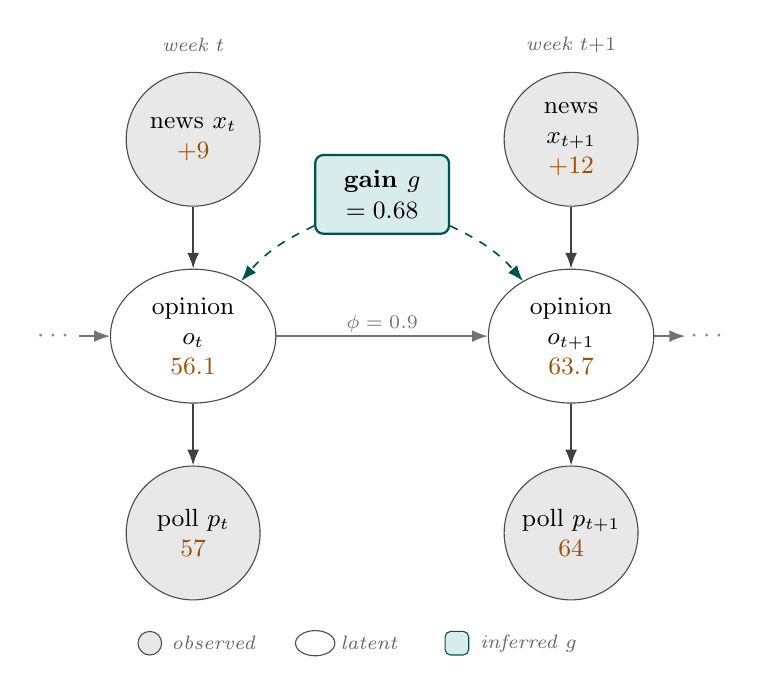
\begin{tikzpicture}[
  >=Latex,
  obs/.style={circle, draw=black!70, fill=gray!18,
              minimum size=1.7cm, text width=1.25cm,
              inner sep=0pt, align=center, font=\small},
  lat/.style={ellipse, draw=black!70, fill=white,
              minimum width=2.1cm, minimum height=1.7cm, text width=1.25cm,
              inner sep=0pt, align=center, font=\small},
  gain/.style={rectangle, rounded corners=3pt, draw=teal!65!black, line width=0.8pt,
               fill=teal!15, minimum width=1.7cm, minimum height=1.0cm,
               inner sep=2pt, align=center, font=\small\bfseries},
  gen/.style={->, semithick, black!75},
  mod/.style={->, semithick, teal!65!black, dashed},
  per/.style={->, semithick, black!55},
  elab/.style={font=\scriptsize, inner sep=1pt},
  slab/.style={font=\scriptsize\itshape, text=black!60}]
% latent gain (the thing to infer); value = this city's hidden truth
\node[gain] (g) at (2.4,1.0) {gain $g$\\$=0.68$};
% one realized instance shown ON the nodes (orange). node fill still encodes observed vs latent.
% chain from baseline o=50: o_t = 50 + 0.68*9 = 56.1; o_{t+1} = 50 + 0.9*6.1 + 0.68*12 = 63.7
\def\val#1{{\color{orange!62!black}\bfseries #1}}
% --- week t ---
\node[obs] (x1) at (0,1.7)    {news $x_t$\\\val{$+9$}};
\node[lat] (o1) at (0,-0.8)   {opinion $o_t$\\\val{$56.1$}};
\node[obs] (p1) at (0,-3.3)   {poll $p_t$\\\val{$57$}};
% --- week t+1 ---
\node[obs] (x2) at (4.8,1.7)   {news $x_{t+1}$\\\val{$+12$}};
\node[lat] (o2) at (4.8,-0.8)  {opinion $o_{t+1}$\\\val{$63.7$}};
\node[obs] (p2) at (4.8,-3.3)  {poll $p_{t+1}$\\\val{$64$}};
% continuity
\node[text=black!45] at (-1.75,-0.8) {$\cdots$};
\node[text=black!45] at (6.55,-0.8)  {$\cdots$};
% within-slice generative edges
\draw[gen] (x1) -- (o1);   \draw[gen] (x2) -- (o2);
\draw[gen] (o1) -- (p1);   \draw[gen] (o2) -- (p2);
% persistence / mean-reversion
\draw[per] (-1.45,-0.8) -- (o1.west);
\draw[per] (o1) -- node[elab,above]{$\phi=0.9$} (o2);
\draw[per] (o2.east) -- (6.25,-0.8);
% g modulates the news->opinion response
\draw[mod] (g) to[bend right=12] (o1);
\draw[mod] (g) to[bend left=12]  (o2);
% time labels
\node[slab] at (0,2.9)   {week $t$};
\node[slab] at (4.8,2.9) {week $t{+}1$};
% legend
\node[circle,draw=black!70,fill=gray!18,minimum size=0.30cm,inner sep=0] at (-0.55,-4.7){};
\node[right,slab] at (-0.40,-4.7){observed};
\node[ellipse,draw=black!70,fill=white,minimum width=0.5cm,minimum height=0.32cm,inner sep=0] at (1.55,-4.7){};
\node[right,slab] at (1.75,-4.7){latent};
\node[rectangle,rounded corners=2pt,draw=teal!65!black,fill=teal!15,minimum size=0.30cm,inner sep=1pt] at (3.35,-4.7){};
\node[right,slab] at (3.52,-4.7){inferred $g$};
\end{tikzpicture}}
\label{fig:exp2}
\vspace{-2em}
\end{wrapfigure}



\subsection{Setup: Task, Forecasters, World}
\label{sec:exp2-setup}

\textbf{Task.}
Each episode is one city tracking a campaign through weekly polls. The city has a hidden \emph{news-responsiveness} parameter \(g\in[0.1,1.0]\), drawn once and never revealed. Each week, the agent observes a news packet \(x_t\) and a noisy poll \(p_t\). Underlying opinion carries over week-to-week, drifting back toward a baseline between shocks (mean-reversion \(\phi\)), so a poll reflects both accumulated past news and the latest packet. Gain, \(g\) sets, for each city, how strongly news moves opinion: low-\(g\) cities are sticky, news barely moves polls; high-\(g\) cities track news nearly one-for-one. Forecasting well, therefore, requires inferring \(g\), the hidden gain that maps visible news into poll movement, while accounting for the persistence that \(g\) acts through. The exact data-generating process and prompts are in App~\ref{app:exp2-prompt}.


\newsavebox{\exptwopromptbox}
\begin{lrbox}{\exptwopromptbox}
\begin{minipage}{0.44\textwidth}
\tiny
\begin{verbatim}
Weekly tracking poll.  Net news is signed
(+ good / - bad); poll = support 0-100.

The city has a FIXED responsiveness g in
[0.1,1.0] (unknown). Each week:
  opinion += about g*news  (+drift ~1)
  poll     = opinion + noise ~2

| Week | Net news | Poll |
|   1  |   -10    |  36  |
|   2  |    +4    |  46  |
|   3  |    -5    |  37  |

Estimate g.  Next news +10: predict the
next poll.  Reply as JSON:
{"points_per_news": _, "predicted_poll": _}
\end{verbatim}
\end{minipage}
\end{lrbox}

\begin{figure}[t]
\centering
\begin{minipage}[c]{0.44\textwidth}
\centering
\setlength{\fboxsep}{5pt}%
\fcolorbox{black!30}{black!4}{\usebox{\exptwopromptbox}}
\end{minipage}\hfill
\begin{minipage}[c]{0.55\textwidth}
\centering
{\setlength{\tabcolsep}{5pt}\renewcommand{\arraystretch}{1.15}%
\begin{tabular}{@{}l c c@{}}
\multicolumn{3}{@{}l@{}}{\itshape\ldots and what each forecaster answers:}\\[2pt]
\toprule
Forecaster & $\hat g$ & next poll\\
\midrule
Bayes oracle & 0.85 & 49\\
\micon{claude.png}~Opus~4.8 & \textcolor{green!72!black}{\textbf{0.90}} & \textcolor{green!72!black}{\textbf{47}}\\
Naive regression & \textcolor{red!72!black}{\textbf{2.07}} & \textcolor{red!72!black}{\textbf{58}}\\
\midrule
\emph{true} ($g{=}0.92$) & 0.92 & ${\approx}50$\\
\bottomrule
\end{tabular}}
\end{minipage}
\caption{\textbf{What the forecaster sees and says.} \emph{(Left)} An abridged prompt (full version, Appendix~\ref{app:exp2-prompt}) for one sparse history from a real city (hidden $g{=}0.92$). The model is \emph{told} the structure and \emph{sees} the news/poll table, but never $g$ or the opinion; the elicitation is neutral. \emph{(Right)} What each forecaster answers: the Bayes oracle and \micon{claude.png}~Opus~4.8 recover $g$ and land near the true next poll, while the naive regression \textcolor{red!72!black}{overshoots} ($\hat g{=}2.07$) on the sparse, noisy history.}
\label{fig:exp2-prompt}
\end{figure}


\textbf{Metrics.} Our claim is about \emph{sparse-evidence judgment}---the carnival-coin picture, where a good prior yields a sensible estimate from a single observation. That is a claim about the \emph{calibration} of one estimate, so we lead with two per-instance \emph{error} metrics, both read as observations accumulate. The first is the recovery error \(\varepsilon_k=\overline{|\hat g_k-g|}\) (lower is better): did the forecaster infer the hidden gain? The second asks whether that inference \emph{pays off in forecasts}---the next-poll error \(\overline{|\hat p_{t+1}-p_{t+1}|}\) (poll points), the mean gap between the poll a forecaster predicts under each held-out shock and the ground-truth expected poll that shock should produce. Because the shocks are counterfactual and never realize, the target is the data-generating process's conditional mean \(\mathbb{E}[p_{t+1}\mid\text{shock}]\), the Bayes-optimal point forecast, so even the oracle, which must filter the current opinion and \(g\), sits above zero (Appendix~\ref{app:exp2-metrics}).

\textbf{References.} We bracket performance with three  baselines. (1) The \emph{Bayes oracle}: grid filtering over \(g\) with a Kalman state update~\citep{kalman1960new}, handed the full generative structure (the \(o_0{=}50\) baseline and mean-reversion \(\phi\)) is the ceiling. (2) The two fixed shortcuts, face value \((\hat g{=}1)\) and ignore news \((\hat g{=}0)\), are the no-inference floor. Between them, (3) the fair statistical bar is a \emph{naive frequentist}: an unregularized through-origin regression of the consecutive poll changes on the news, using only what the agent sees. A forecaster that infers structure should beat the shortcuts and the frequentist.



We evaluate frontier agents and open-weight local models with the same multi-shock probe at every prefix: open-weight models on 250 shared-seed cities, the frontier agents on \(n{=}100\). After \(k\) observed weeks, each model estimates the per-news response and predicts the next poll under the four shocks, yielding \(\hat g_k\).


\subsection{Results: Calibrated Sparse-Evidence Inference}
\label{sec:exp2-results}

\begin{figure*}[t]
\centering
\includegraphics[width=\linewidth]{figures/exp2_skill.pdf}
\caption{\textbf{Frontier agents recover the hidden gain and forecast the next poll near-optimally---from a single week.} Both panels read \emph{error} as the observed history grows (weeks $k$), against the same bracket: the Bayes-oracle ceiling, the overshooting naive frequentist, and the two fixed shortcuts (face value, ignore news).
\emph{(A) Latent recovery.} Error $\varepsilon_k{=}\overline{|\hat g_k-g|}$ on the hidden gain (lower is better).
\emph{(B) Forecast skill.} Next-poll error $\overline{|\hat p_{t+1}-p_{t+1}|}$ (poll points) under the four held-out shocks, scored against the ground-truth expected poll.  Only the three frontier agents are shown here for legibility; the full open-weight roster ($n{=}68$--$250$) orders by scale in App. Table~\ref{tab:exp2-poll} and Fig.~\ref{fig:exp2-informativeness}. Frontier $n{=}100$.}
\label{fig:exp2-skill}
\vspace{-1em}
\end{figure*}

\begin{wraptable}{r}{0.50\textwidth}
\centering
\vspace{-2em}
\setlength{\tabcolsep}{2pt}
\caption{Forecast skill from a sparse history.  Each $k$ pairs the two errors of Fig.~\ref{fig:exp2-skill} (both lower is better): the \emph{latent-recovery} error $\varepsilon_k{=}\overline{|\hat g-g|}$ and the \emph{next-poll} error $\pi_k{=}\overline{|\hat p_{t+1}-p_{t+1}|}$ (poll points).  Cells are \textcolor{green!62!black}{green} where a model beats the frequentist on that metric, \textcolor{red!62!black}{red}  where it falls short. The frontier agents beat the frequentist on both metrics from a single week.  Frontier $n{=}100$; open-weight $n=250$.
\textsuperscript{$\dagger$}Frontier probe.}
\label{tab:exp2-skill}
\footnotesize
\begin{tabular}{l@{\hskip 5pt}cc cc cc cc}
\toprule
 & \multicolumn{2}{c}{$k{=}1$} & \multicolumn{2}{c}{$k{=}2$} & \multicolumn{2}{c}{$k{=}3$} & \multicolumn{2}{c}{$k{=}5$} \\
\cmidrule(lr){2-3}\cmidrule(lr){4-5}\cmidrule(lr){6-7}\cmidrule(lr){8-9}
\textbf{Forecaster} & $\varepsilon{\downarrow}$ & $\pi{\downarrow}$ & $\varepsilon{\downarrow}$ & $\pi{\downarrow}$ & $\varepsilon{\downarrow}$ & $\pi{\downarrow}$ & $\varepsilon{\downarrow}$ & $\pi{\downarrow}$ \\
\midrule
Bayes oracle & .18 & 1.9 & .15 & 1.6 & .14 & 1.5 & .10 & 1.2 \\
Naive freq. & .46 & 3.9 & .35 & 3.1 & .24 & 2.6 & .16 & 2.2 \\
\midrule
\micon{claude.png}~Opus~4.8\textsuperscript{$\dagger$} & \cellcolor{green!22}.20 & \cellcolor{green!22}2.4 & \cellcolor{green!22}.18 & \cellcolor{green!22}2.4 & \cellcolor{green!22}.18 & \cellcolor{green!22}2.4 & \cellcolor{green!22}.13 & \cellcolor{green!22}2.0 \\
\micon{openai.png}-5.4\textsuperscript{$\dagger$} & \cellcolor{green!22}.20 & \cellcolor{green!22}2.4 & \cellcolor{green!22}.22 & \cellcolor{green!22}2.5 & \cellcolor{green!22}.19 & \cellcolor{green!22}2.4 & \cellcolor{green!22}.15 & \cellcolor{green!22}2.0 \\
\micon{deepseek.png}~V4-Pro\textsuperscript{$\dagger$} & \cellcolor{green!22}.22 & \cellcolor{green!22}2.5 & \cellcolor{green!22}.24 & \cellcolor{green!22}2.7 & \cellcolor{green!22}.18 & \cellcolor{green!22}2.3 & \cellcolor{green!22}.14 & \cellcolor{green!22}2.1 \\
\midrule
\micon{llamma.pdf}~3.1-70B & \cellcolor{green!22}.23 & \cellcolor{green!22}2.9 & \cellcolor{green!22}.23 & \cellcolor{green!22}2.7 & \cellcolor{green!22}.21 & \cellcolor{red!18}2.6 & \cellcolor{red!18}.17 & \cellcolor{red!18}2.4 \\
\micon{qwen.pdf}~2.5-32B & \cellcolor{green!22}.26 & \cellcolor{green!22}3.0 & \cellcolor{green!22}.23 & \cellcolor{green!22}2.5 & \cellcolor{green!22}.20 & \cellcolor{green!22}2.5 & \cellcolor{red!18}.16 & \cellcolor{red!18}2.3 \\
\micon{qwen.pdf}~2.5-14B & \cellcolor{green!22}.28 & \cellcolor{green!22}3.3 & \cellcolor{green!22}.25 & \cellcolor{green!22}2.9 & \cellcolor{green!22}.20 & \cellcolor{red!18}2.7 & \cellcolor{red!18}.20 & \cellcolor{red!18}2.5 \\
\micon{llamma.pdf}~3.1-8B & \cellcolor{red!18}.95 & \cellcolor{red!18}10.3 & \cellcolor{red!18}.61 & \cellcolor{red!18}7.1 & \cellcolor{red!18}.50 & \cellcolor{red!18}6.3 & \cellcolor{red!18}.60 & \cellcolor{red!18}6.9 \\
\micon{qwen.pdf}~2.5-7B & \cellcolor{green!22}.31 & \cellcolor{green!22}3.5 & \cellcolor{green!22}.27 & \cellcolor{green!22}2.9 & \cellcolor{green!22}.23 & \cellcolor{red!18}2.9 & \cellcolor{red!18}.23 & \cellcolor{red!18}3.1 \\
\bottomrule
\end{tabular}
\vspace{-2em}
\end{wraptable}

The agents recover latent structure and turn it into forecasts, and---crucially---do both \emph{calibratedly from sparse evidence} (Figure~\ref{fig:exp2-skill}): from a single week their implied gain sits near the Bayes-optimal estimate and their next-poll forecasts land within \({\approx}2\) points of ground truth, both far better than every fixed shortcut and, in the sparse regime, better than an unregularized regression that overshoots. But the edge is one of \emph{regularization, not omniscience}---they approximate optimal Bayesian shrinkage rather than exceeding it, so once a few observations accumulate a matched statistical estimator catches them.

\textbf{Calibrated from a single week---on both errors.} The references bracket the task (Table~\ref{tab:exp2-skill}): the fixed shortcuts sit far off ($\varepsilon{\approx}.46$--$.54$, $\pi{\approx}3.9$--$4.3$) and the Bayes oracle is the ceiling ($\varepsilon{=}.10$--$.18$, $\pi{=}1.2$--$1.9$). From one poll the frontier agents already sit near the oracle---$\varepsilon_1{\approx}.20$, next-poll error ${\approx}2.4$ points---and beat the fair statistical bar on \emph{both} metrics at every $k$. The naive frequentist cannot identify $g$ from a single poll, so it reads the news at face value ($\varepsilon_1{\approx}.46$) then \emph{overshoots} on one or two noisy points ($\varepsilon_2{\approx}.35$, $\pi_2{\approx}3.1$); the agents' prior regularizes where the bare fit does not. No prompt hint tells them how to treat the sparse history (Appendix~\ref{app:exp2-prompt}), so this is their own disposition---the carnival-coin picture, measured.

\textbf{Regularization, not omniscience.} The edge is bounded: the agents approximate optimal Bayesian shrinkage, so a matched estimator catches them as data accumulates ($k{=}5$: agents $\varepsilon{\approx}.13$--$.15$, frequentist $.16$, oracle $.10$). Low error alone is also not enough---guessing the prior mean is calibrated ($\varepsilon{=}.22$) yet \emph{blind} ($\rho{=}0$; Appendix Fig.~\ref{fig:exp2-informativeness}); only the agents are both calibrated and informative. Recovery still orders by capability: the frontier agents are calibrated in magnitude ($\overline{\hat g}{\approx}.55$--$.58$ vs.\ true $.55$) with a \emph{stated} rate that tracks behavior (stated-$\rho{\approx}.7$--$.77$), while the smallest read news near face value ($\varepsilon{>}.5$) and cannot articulate $g$ (Appendix~\ref{app:exp2-parity-refs}).

\textbf{Takeaway.} In a world where the hidden state is known, agents' forecasts vary systematically with it and are \emph{calibrated from a single week}---recovering the gain and forecasting the next poll to ${\approx}2$ points, beating every shortcut and an unregularized regression exactly in the sparse regime real forecasting inhabits, because a useful prior regularizes where a bare estimator overshoots. But the edge is regularization, not omniscience: a matched estimator catches them once data accumulates. This motivates Experiment~3: whether training can push agents to \emph{beat}, not just match, a well-posed estimator, and transfer beyond the training distribution.

% ------------------------------------------------------------------
\section{Experiment 2: Recovering Hidden Structure in a Simulated Forecasting World}
\label{sec:exp2}
% ------------------------------------------------------------------



\section{Experiment 3: Training and Transfer Across Synthetic and Real Forecasting Worlds}

Experiments~1 and~2 treated inductive world-modeling as a \emph{fixed} property of an agent: a
disposition we probe but do not change.
In Experiment~2 the strongest agents recovered the hidden gain from a single
observation but \emph{plateaued}: they reached, yet never cleared, a well-posed same-information
forecaster.
Experiment~3
asks whether \emph{forecasting training} can move that ceiling, and moreover, whether any gain is a general improvement in inductive world-modeling rather than fit to the trained distribution.
Transfer is the discriminating test: we train on one family of forecasting problems and evaluate on held-out families the agent never saw, reusing the same diagnostics of Experiments~1 and~2.

\subsection{Synthetic worlds: training latent recovery and testing it on a held-out world}
\label{sec:exp3-synthetic}

\textbf{A family of latent-structure worlds.}  We generalize the Experiment~2 world into a
\emph{family} of small linear-Gaussian DAGs that share its logic but vary its structure
(Fig.~\ref{fig:exp3-heldout}).  In each, observed news $x$ drives a latent opinion $o$ that carries over
and mean-reverts week to week and emits an observed poll $p$; a single
edge---the \emph{hidden gain} $g$, drawn once per city---sets how strongly news moves opinion and is
never revealed.  The $20$ structures vary everything \emph{around} that gain: the number of news
drivers, the depth and delay of the news$\to$poll path (direct, two-stage, three-stage, lagged),
confounding latents, multiple polls, and which edge is hidden (an input gain, an inter-latent coupling,
or a persistence).  The shared task is always the same---forecast next week's poll---and the forecaster
sees only the news/poll history: the graph, the number of latent stages, and the gain are all hidden,
so it must \emph{infer} the response from data.  A per-structure Kalman filter that marginalizes $g$ is
the optimal forecaster (the oracle), computable for any linear-Gaussian DAG.

% Experiment 3 — the forecasting family (5 of 20 linear-Gaussian DAG structures).
% Requires: \usetikzlibrary{shapes.geometric,arrows.meta,positioning} and xcolor (teal).
\tikzset{
  obs/.style={circle, draw=black!70, fill=gray!16, minimum size=0.66cm,
              inner sep=0pt, font=\small},
  lat/.style={ellipse, draw=black!70, fill=white, minimum width=0.9cm,
              minimum height=0.66cm, inner sep=0pt, font=\small},
  gain/.style={rectangle, rounded corners=2pt, draw=teal!65!black, line width=0.7pt,
               fill=teal!12, inner sep=2.2pt, font=\scriptsize\bfseries, text=teal!65!black},
  kn/.style={-{Latex[length=4.5pt]}, semithick, black!72},      % known edge
  inh/.style={-{Latex[length=5pt]}, line width=1.7pt, black!82},% inhibitory (thick)
  hid/.style={-{Latex[length=4.5pt]}, thick, teal!65!black, dashed}, % hidden gain
  per/.style={-{Latex[length=3.5pt]}, thin, black!42},          % phi self-loop
  ttl/.style={font=\small\bfseries, text=black!82},             % panel title
}
\newcommand{\sll}[1]{\draw[per] (#1) to[out=158,in=202,looseness=5.2] (#1);} % left loop
\newcommand{\slr}[1]{\draw[per] (#1) to[out=22,in=-22,looseness=5.2] (#1);}  % right loop
\def\vs{1.08} % vertical spacing between stacked nodes

% ---- TRAINING WORLDS (9) -------------------------------------------
\newcommand{\dHiddenPhi}{%
  \node[obs] (x) at (0,0) {$x$};   \node[lat] (o) at (0,-\vs) {$o$};
  \node[obs] (p) at (0,-2*\vs) {$p$};   \node[gain] (g) at (1.15,-0.55) {$g$};
  \draw[kn](x)--(o); \draw[kn](o)--(p); \draw[hid](g) to[bend right=12] (o); \slr{o}
  \node[ttl] at (0,-2*\vs-0.85) {Hidden $\phi$};}

\newcommand{\dChainTwo}{%
  \node[obs] (x) at (0,0) {$x$};   \node[lat] (o1) at (0,-\vs) {$o_1$};
  \node[lat] (o2) at (0,-2*\vs) {$o_2$};   \node[obs] (p) at (0,-3*\vs) {$p$};
  \node[gain] (g) at (1.15,-0.55) {$g$};
  \draw[kn](x)--(o1); \draw[kn](o1)--(o2); \draw[kn](o2)--(p);
  \draw[hid](g) to[bend right=12] (o1); \sll{o1}\sll{o2}
  \node[ttl] at (0,-3*\vs-0.85) {Chain-2};}

\newcommand{\dChainTwoH}{%
  \node[obs] (x) at (0,0) {$x$};   \node[lat] (o1) at (0,-\vs) {$o_1$};
  \node[lat] (o2) at (0,-2*\vs) {$o_2$};   \node[obs] (p) at (0,-3*\vs) {$p$};
  \node[gain] (g) at (1.15,-2*\vs+0.55) {$g$};
  \draw[kn](x)--(o1); \draw[kn](o1)--(o2); \draw[kn](o2)--(p);
  \draw[hid](g) to[bend left=12] (o2); \sll{o1}\sll{o2}
  \node[ttl] at (0,-3*\vs-0.85) {Chain-2 (hidden $\phi$)};}

\newcommand{\dEcho}{%
  \node[obs] (x) at (0,0) {$x$};   \node[lat] (o1) at (-0.95,-1.2) {$o_1$};
  \node[lat] (o2) at (0.95,-1.2) {$o_2$};   \node[obs] (p) at (-0.95,-2.5) {$p$};
  \node[gain] (g) at (-2.05,-0.5) {$g$};
  \draw[kn](x)--(o1); \draw[kn](x)--(o2); \draw[kn](o2) to[bend left=14] (o1);
  \draw[kn](o1)--(p); \draw[hid](g) to[bend right=12] (o1); \sll{o1}\slr{o2}
  \node[ttl] at (0,-3.35) {Echo};}

\newcommand{\dInhibitory}{%
  \node[obs] (x) at (0,0) {$x$};   \node[lat] (o1) at (0,-\vs) {$o_1$};
  \node[lat] (o2) at (0,-2*\vs) {$o_2$};   \node[obs] (p) at (0,-3*\vs) {$p$};
  \node[gain] (g) at (1.15,-0.55) {$g$};
  \draw[kn](x)--(o1); \draw[inh](o1)--(o2); \draw[kn](o2)--(p);
  \draw[hid](g) to[bend right=12] (o1); \sll{o1}\sll{o2}
  \node[ttl] at (0,-3*\vs-0.85) {Inhibitory};}

\newcommand{\dLagged}{%
  \node[obs] (x) at (0,0) {$x$};   \node[lat] (o2) at (0,-\vs) {$o_2$};
  \node[lat] (o1) at (0,-2*\vs) {$o_1$};   \node[obs] (p) at (0,-3*\vs) {$p$};
  \node[gain] (g) at (-1.5,-2*\vs+0.55) {$g$};
  \draw[kn](x)--(o2); \draw[kn](o2)--(o1); \draw[kn](o1)--(p);
  \draw[hid](g) to[bend left=12] (o1); \slr{o2}\slr{o1}
  \node[ttl] at (0,-3*\vs-0.85) {Lagged};}

\newcommand{\dSkip}{%
  \node[obs] (x) at (0,0) {$x$};   \node[lat] (o1) at (0,-\vs) {$o_1$};
  \node[lat] (o2) at (0,-2*\vs) {$o_2$};   \node[obs] (p) at (0,-3*\vs) {$p$};
  \node[gain] (g) at (1.15,-0.55) {$g$};
  \draw[kn](x)--(o1); \draw[kn](o1)--(o2); \draw[kn](o2)--(p);
  \draw[kn](x) to[out=200,in=160,looseness=1.25] (o2);   % skip edge x->o2
  \draw[hid](g) to[bend right=12] (o1); \slr{o1}\slr{o2}
  \node[ttl] at (0,-3*\vs-0.85) {Skip};}

\newcommand{\dChainThree}{%
  \node[obs] (x) at (0,0) {$x$};   \node[lat] (o1) at (0,-\vs) {$o_1$};
  \node[lat] (o2) at (0,-2*\vs) {$o_2$};   \node[lat] (o3) at (0,-3*\vs) {$o_3$};
  \node[obs] (p) at (0,-4*\vs) {$p$};   \node[gain] (g) at (1.15,-0.55) {$g$};
  \draw[kn](x)--(o1); \draw[kn](o1)--(o2); \draw[kn](o2)--(o3); \draw[kn](o3)--(p);
  \draw[hid](g) to[bend right=12] (o1); \sll{o1}\sll{o2}\sll{o3}
  \node[ttl] at (0,-4*\vs-0.85) {Chain-3};}

\newcommand{\dTwoNewsSplit}{%
  \node[obs] (x1) at (-0.95,0) {$x_1$};   \node[obs] (x2) at (0.95,0) {$x_2$};
  \node[lat] (o1) at (-0.95,-1.2) {$o_1$};   \node[lat] (o2) at (0.95,-1.2) {$o_2$};
  \node[obs] (p) at (-0.95,-2.5) {$p$};   \node[gain] (g) at (-2.15,-0.5) {$g$};
  \draw[kn](x1)--(o1); \draw[kn](x2)--(o2); \draw[kn](o2) to[bend left=14] (o1);
  \draw[kn](o1)--(p); \draw[hid](g) to[bend right=12] (o1); \sll{o1}\slr{o2}
  \node[ttl] at (0,-3.35) {Two-news split};}

% ---- HELD-OUT WORLDS (4) -------------------------------------------
\newcommand{\dDirect}{%
  \node[obs] (x) at (0,0) {$x$};   \node[lat] (o) at (0,-\vs) {$o$};
  \node[obs] (p) at (0,-2*\vs) {$p$};   \node[gain] (g) at (1.15,-0.55) {$g$};
  \draw[kn](x)--(o); \draw[kn](o)--(p); \draw[hid](g) to[bend right=12] (o); \slr{o}
  \node[ttl] at (0,-2*\vs-0.85) {Direct};}

\newcommand{\dChainFour}{%
  \node[obs] (x) at (0,0) {$x$};   \node[lat] (o1) at (0,-\vs) {$o_1$};
  \node[lat] (o2) at (0,-2*\vs) {$o_2$};   \node[lat] (o3) at (0,-3*\vs) {$o_3$};
  \node[lat] (o4) at (0,-4*\vs) {$o_4$};   \node[obs] (p) at (0,-5*\vs) {$p$};
  \node[gain] (g) at (1.15,-0.55) {$g$};
  \draw[kn](x)--(o1); \draw[kn](o1)--(o2); \draw[kn](o2)--(o3);
  \draw[kn](o3)--(o4); \draw[kn](o4)--(p);
  \draw[hid](g) to[bend right=12] (o1); \sll{o1}\sll{o2}\sll{o3}\sll{o4}
  \node[ttl] at (0,-5*\vs-0.85) {Chain-4};}

\newcommand{\dMediators}{%
  \node[obs] (x) at (0,0) {$x$};   \node[lat] (o1) at (-1.0,-1.2) {$o_1$};
  \node[lat] (o2) at (1.0,-1.2) {$o_2$};   \node[lat] (o3) at (0,-2.45) {$o_3$};
  \node[obs] (p) at (0,-3.7) {$p$};   \node[gain] (g) at (-2.1,-0.5) {$g$};
  \draw[kn](x)--(o1); \draw[kn](x)--(o2); \draw[kn](o1)--(o3);
  \draw[kn](o2)--(o3); \draw[kn](o3)--(p);
  \draw[hid](g) to[bend right=12] (o1); \sll{o1}\slr{o2}\slr{o3}
  \node[ttl] at (0,-4.55) {Mediators};}

\newcommand{\dTwoNewsFeedback}{%
  \node[obs] (x1) at (-1.0,0) {$x_1$};   \node[obs] (x2) at (1.0,0) {$x_2$};
  \node[lat] (o1) at (-1.0,-1.25) {$o_1$};   \node[lat] (o2) at (1.0,-1.25) {$o_2$};
  \node[obs] (p) at (-1.0,-2.6) {$p$};   \node[gain] (g) at (-2.2,-0.5) {$g$};
  \draw[kn](x1)--(o1); \draw[kn](x2)--(o2);
  \draw[kn](o1) to[bend left=16] (o2); \draw[kn](o2) to[bend left=16] (o1);
  \draw[kn](o1)--(p); \draw[hid](g) to[bend right=12] (o1); \sll{o1}\slr{o2}
  \node[ttl] at (0,-3.45) {Two-news feedback};}


% ------------- 2. MAIN-TEXT FIGURE: held-out worlds ------------------
\begin{figure}[t]
\centering
\resizebox{\linewidth}{!}{%
\begin{tikzpicture}
  \begin{scope}[shift={(0,0)}]     \dDirect          \end{scope}
  \begin{scope}[shift={(3.4,0)}]   \dChainFour       \end{scope}
  \begin{scope}[shift={(7.6,0)}]   \dMediators       \end{scope}
  \begin{scope}[shift={(11.8,0)}]  \dTwoNewsFeedback \end{scope}
  % legend
  \begin{scope}[shift={(15.2,-2.1)},font=\scriptsize]
    \node[circle,draw=black!70,fill=gray!16,minimum size=0.4cm,inner sep=0] at (0,1.35) {};
    \node[right] at (0.3,1.35) {observed ($x$ news, $p$ poll)};
    \node[ellipse,draw=black!70,fill=white,minimum width=0.55cm,minimum height=0.4cm,inner sep=0] at (0,0.72) {};
    \node[right] at (0.3,0.72) {latent opinion $o$};
    \node[gain,minimum size=0.34cm] at (0,0.08) {$g$};
    \node[right] at (0.3,0.08) {hidden gain $g$ (infer from polls)};
    \draw[per] (-0.2,-0.7) to[out=158,in=202,looseness=5] (-0.2,-0.5);
    \node[right] at (0.3,-0.6) {$\phi$: carry-over / mean-reversion};
    \draw[kn] (-0.24,-1.28) -- (0.24,-1.28);
    \node[right] at (0.3,-1.28) {known edge};
  \end{scope}
\end{tikzpicture}}
\caption{\textbf{Held-out transfer worlds (4).} These latent-opinion structures are never seen during
training and are used only to evaluate transfer: \emph{Direct} (the Experiment-2 world), a deeper
\emph{Chain-4}, a fork--join \emph{Mediators} graph, and \emph{Two-news feedback} with two news
drivers and a bidirectional $o_1\!\leftrightarrow\!o_2$ coupling. In every world, observed news $x$
drives a dynamic latent opinion $o$ (self-loop $\phi$) that emits an observed poll $p$; the
\textcolor{teal!65!black}{hidden gain $g$} is drawn once per city and must be inferred from the polls
alone. The task is always to forecast next week's poll. See App.~\ref{app:exp3} for training world DAGs.}

\label{fig:exp3-heldout}
\end{figure}


\textbf{Metrics and references.}  We reuse the two Experiment~2 errors, read by the same four-shock
predict-then-slope probe: the \emph{next-poll forecast error} $\overline{|\hat p_{t+1}-p_{t+1}|}$ (poll
points; universal across structures) and, where a one-step input$\to$output gain is defined, the
\emph{recovery error} $\overline{|\hat g-g|}$.  Three references bracket any forecaster: the
\emph{oracle} (knows the structure, infers $g$) is the ceiling; a \emph{naive frequentist} (an
unregularized, structure-agnostic data fit) is the fair statistical bar; and \emph{persistence}
(predict the last poll) is the no-inference floor.  A forecaster that knows nothing of the structure
sits between persistence and the oracle, and its position measures how much structure it infers from
data alone.

\textbf{Training and the transfer test.}  We split the family into $16$ \emph{training} structures and
$4$ \emph{held-out} ones; among the held-out is the direct chain---the Experiment~2 world itself---so
the test literally asks whether training on other structures improves recovery on the Experiment~2
world.  We train Qwen-3-4B (LoRA rank $32$) with Dr.\ GRPO on the forecast-accuracy reward over the $16$
training structures; the model never observes the graph or $g$ and only ever outputs a next-poll
forecast, so improving the reward is possible only by inferring the response.  The decisive measure is
\emph{transfer across structure}: we evaluate on the $4$ held-out structures the model never trained
on, with the identical instrument. A gain there---beyond new cities of a trained structure---is
evidence that training reshaped a \emph{general} inductive bias rather than fitting one structure's
parameters.

\textbf{Result: training on other structures transfers to held-out ones.}
Table~\ref{tab:exp3-transfer} reports before (untrained) and after ($60$ Dr.\ GRPO steps) on the four
held-out structures.  Training improves \emph{every one} and moves the held-out means the right way on
both metrics: forecast error falls from $5.20$ to $3.73$ poll points ($-28\%$) and recovery error from
$.42$ to $.24$ ($-43\%$).  The effect is exactly the \emph{regularization} Experiment~2 predicts.  The
untrained model \emph{over-reads} news---its implied gain is far too high, so its recovery error
($.42$) is worse than every statistical floor and it forecasts no better than persistence.  Training
pulls the implied gain down toward the truth, so recovery lands at $.24$ (near the no-information prior,
below the naive frequentist) and forecast error drops below the naive statistical bar.  As in
Experiment~2, the edge is bounded: the trained model closes roughly half the gap to the oracle
($\approx1.7$ / $.14$) rather than reaching it.  So training buys an improvement in inductive
world-modeling that \emph{transfers to structures never seen in training}---but shrinkage toward the
optimal estimate, not past it.

\begin{table}[h]
\centering
\caption{Synthetic arm --- \textbf{transfer across structure}.  Qwen-3-4B before (untrained) and after
$60$ Dr.\ GRPO steps on the $16$ \emph{training} structures, evaluated on the $4$ \emph{held-out}
structures it never trained on, with the Experiment~2 four-shock instrument.  Both errors are
lower-is-better: next-poll forecast error $\overline{|\hat p_{t+1}-p_{t+1}|}$ (poll points) and, where a
one-step gain exists, recovery error $\overline{|\hat g-g|}$.  Reference bracket: oracle $\approx1.7$ /
$.14$, naive frequentist $\approx3.85$ / $.37$, persistence $\approx4.6$.  Training improves every
held-out structure on both axes; the gain is regularization of the base model's over-reading, closing
about half the gap to the oracle. ($60$-step LoRA pilot, single seed; longer and multi-seed runs in
progress.)}
\label{tab:exp3-transfer}
\footnotesize
\begin{tabular}{l cc}
\toprule
Held-out structure & forecast err (base$\to$trained) & recovery err (base$\to$trained) \\
\midrule
direct chain (the Exp-2 world)        & $4.30 \to 2.91$ & $.41 \to .23$ \\
hidden-persistence                    & $4.11 \to 3.18$ & --- \\
three-stage delay                     & $7.48 \to 5.41$ & --- \\
opposed drivers                       & $4.89 \to 3.43$ & $.44 \to .26$ \\
\midrule
\textbf{held-out mean}                & $\mathbf{5.20 \to 3.73}$ & $\mathbf{.42 \to .24}$ \\
\bottomrule
\end{tabular}
\end{table}


% ------------------------------------------------------------------
\subsection{Real-world pastcasting: training coherent updating and testing it on held-out questions}
\label{sec:exp3-pastcasting}
% ------------------------------------------------------------------


\textbf{Setup.}  The pastcasting arm reuses the Experiment~1 pipeline: the same structured forecast (event model, competing hypotheses $H_1/H_2$, headline $\hat p = P(H_1)$) and the same agents. However, we use \emph{resolved} historical Polymarket questions, restricting each agent to evidence available at the time.
This closes the one gap Experiment~1 had to defer: with realized outcomes in hand we can compute a genuine accuracy reward (Brier / log-loss against resolution), the ``resolution follow-up'' flagged in Appendix~\ref{app:exp1-limitations}.
We train on one family of questions and evaluate on a held-out set, so the score measures forecasting skill that generalizes across questions, not memorization of particular resolutions.

\section{Related Work}
\label{related_work}

\textbf{Judgmental forecasting and superforecasting.}
Human forecasts of uncertain events are often poorly calibrated~\citep{tetlock2005expert}, but tournament research isolates the practices that distinguish the best forecasters---decomposition, base-rate use, aggregation, and incremental updating~\citep{mellers2014psychological,tetlock2016superforecasting}.
Related work treats judgment as indispensable but bias-prone in demand forecasting~\citep{lawrence2006judgmental}.
We operationalize several of these practices as diagnostics for language agents.

\textbf{LLMs and forecasting.}
\citet{zou2022forecasting} benchmark leakage-free LM forecasting against human crowds, and recent systems approach competitive performance via retrieval~\citep{halawi2024approaching} and model ensembling~\citep{schoenegger2024wisdom}.
Whether this accuracy reflects event-specific reasoning or aggregation and retrieval over training distributions is what our diagnostics target.

\textbf{World models in language agents.}
In machine learning, a ``world model'' classically denotes a learned latent-dynamics model for prediction and control~\citep{ha2018world,lecun2022path}.
In the language setting, probing suggests emergent structure, e.g. board state in an Othello model~\citep{li2023emergent}, or latent agent properties behind text~\citep{andreas2022agent}.
However, skeptics note that current systems lack human-like causal models~\citep{mitchell2023ai}, and \citet{vafa2025foundation} show that strong predictions can coexist with a wrong, non-transferable latent model.
We treat this as an empirical question about forecasting agents.

\textbf{Evaluation beyond accuracy.}
Held-out accuracy overstates competence, motivating behavioral tests~\citep{ribeiro2020beyond}, consistency checks~\citep{elazar2021measuring}, and calibration~\citep{brier1950verification}.
Our metrics combine these: directional counterfactual interventions test coherent updating, a sensitivity ratio tests causal selectivity, and transfer tests probe generalization beyond the training distribution~\citep{vafa2025foundation}.


\section{Conclusion}

Across unresolved real-world markets, controlled synthetic worlds, and preliminary training experiments, our results suggest that strong language agents do more than imitate surface patterns or copy market prices. They update forecasts coherently in response to causally relevant evidence, largely ignore orthogonal evidence, and, in controlled environments, infer hidden latent structure from sparse observations. These abilities are strongest in frontier systems and weaker but still partially present in larger open-weight models.

At the same time, the evidence points to partial rather than complete world modeling. In the simulated forecasting world, frontier agents are most impressive in the sparse-data regime, where useful priors allow them to approximate Bayes-optimal shrinkage from very few observations. But once enough data accumulates, a matched statistical estimator catches up or overtakes them. This suggests that current agents possess useful inductive biases for judgmental forecasting, especially when evidence is scarce, while still falling short of optimal latent-state inference.

\bibliographystyle{iclr2026_conference}
\bibliography{iclr2026/iclr2026_conference}

% ============================================================
%  APPENDIX A — EXPERIMENT 1 FULL DETAILS
%  Place after the main body, e.g. \appendix\section{...}
% ============================================================

% ============================================================
%  APPENDIX A — EXPERIMENT 1 FULL DETAILS  (revised 2026-06-16)
%  Place after the main body, e.g. \appendix\section{...}
% ============================================================

\section{Experiment 1: Full Experimental Details}
\label{app:exp1}

\subsection{Market Selection}
\label{app:market-selection}

We query the Polymarket REST API for all binary markets satisfying the following filters
as of June~9, 2026 (the primary sampling date):

\begin{itemize}
  \item \textbf{Status}: market is open (not yet resolved or expired).
  \item \textbf{Closing window}: resolution date between 14 and 180 days from sampling date.
  \item \textbf{Volume}: CLOB transaction count $\geq 1{,}000$.
  \item \textbf{Category}: one of Politics, Government, Elections, Economics, Geopolitics.
\end{itemize}

This produces a candidate pool from which we draw 100~markets for the primary study,
maximising category, market-price, and topic-type diversity.  An extended set of 20
additional markets sampled on June~11--14 brings the total pool to 120~markets; local
models (Qwen~2.5 and Llama families) were run on all 120~markets.
Frontier models (Claude Opus~4.8, DeepSeek V4-Pro) were run on the original 100-market
set; GPT-5.4 was run on 92 of these markets (June~5 pilot selection) and its
Stage~3 records target that subset.

Daily CLOB price histories for all pool markets are collected (Polymarket CLOB API,
1-day fidelity, up to 28-day rolling windows) to support calibration analysis and
price-history visualizations in the interactive viewer.

\begin{table}[h]
\centering
\caption{Sample pilot markets from the Experiment~1 pool.  ``Mid'' is the Polymarket
best-bid mid-price at the time of agent elicitation.}
\label{tab:markets}
\small
\begin{tabular}{p{6.2cm} l c}
\toprule
\textbf{Question} & \textbf{Category} & \textbf{Mid} \\
\midrule
Strait of Hormuz traffic returns to normal by end of June? & Geopolitics & 0.17 \\
US--Iran nuclear deal by June~30?                          & Middle East & 0.28 \\
US $\times$ Iran permanent peace deal by July~31, 2026?    & Iran        & 0.41 \\
Will Renan Santos win the 2026 Brazilian presidential election? & Brazil  & 0.16 \\
Will Tom Steyer win the California Governor Election in 2026?   & Elections & 0.22 \\
\bottomrule
\end{tabular}
\end{table}

\subsection{Frontier Agents (Azure AI Foundry)}
\label{app:agent-arch-frontier}

All three frontier models are deployed via Microsoft Azure AI~Foundry using the
Responses~API protocol (\texttt{client.responses.create} with
\texttt{previous\_response\_id} for multi-turn context chaining).  Web search is
provided natively by the Azure AI~Foundry agent runtime; each turn that requests
research issues Bing-backed searches and receives summarised web content before the
model produces its response.

\begin{itemize}
  \item \textbf{GPT-5.4}: deployed as \texttt{forecasting-agent}, version~2; accessed at
        the Azure AI~Foundry project endpoint.  Runs the standard four-turn protocol
        (T1: event model; T2: web research; T3: red/blue-team steelman; T4: structured
        JSON).

  \item \textbf{Claude Opus~4.8} (\texttt{claude-opus-4-8}): deployed as
        \texttt{forecasting-agent-2}, version~2.  Due to an Azure-side constraint that
        limits accumulated context to three chained turns before a 400-error
        (\texttt{invalid\_request\_error}), we run Claude in three-turn mode
        (T1: event model; T2: web research; T3: structured JSON), omitting the optional
        red/blue-team deepening turn.

  \item \textbf{DeepSeek V4-Pro} (\texttt{deepseek-r1}): deployed as
        \texttt{deep-seek-forecast}, version~2.  Runs the same four-turn protocol as
        GPT-5.4 with the red/blue-team turn included.
\end{itemize}

All three frontier agents use the same prompt templates to preserve within-experiment
comparability (see Section~\ref{app:prompts}).

\subsection{Local Agents (Ollama)}
\label{app:agent-arch-local}

Local models are served via Ollama on cluster GPU nodes.  All seven local models share
the same Stage~1 prompt templates as frontier models; the key differences are:

\begin{itemize}
  \item \textbf{No web search}: local models receive the question text only, with no
        retrieval turn.  Stage~1 collapses to a single structured-output generation call.
  \item \textbf{Output scale}: smaller models (7--8B) tend to output raw probability
        values on a 0--100 scale rather than the 0--1 float specified in the schema.
        These values are normalised in post-processing before metric computation.
  \item \textbf{Temperature}: all local models run at temperature 0.7 with top-p 0.95.
\end{itemize}

The seven local models with their parameter counts and Ollama tags are:

\begin{table}[h]
\centering
\caption{Local models run via Ollama.  ``Params'' is nominal parameter count.  Stage~3
complete indicates whether counterfactual update records are available (as of 2026-06-15).}
\label{tab:local-models}
\small
\begin{tabular}{lllc}
\toprule
\textbf{Model} & \textbf{Ollama tag} & \textbf{Params} & \textbf{Stage~3 complete} \\
\midrule
Qwen~2.5-7B    & \texttt{qwen2.5:7b}    & 7B  & \checkmark \\
Qwen~2.5-14B   & \texttt{qwen2.5:14b}   & 14B & \checkmark \\
Qwen~2.5-32B   & \texttt{qwen2.5:32b}   & 32B & \checkmark \\
Qwen~2.5-72B   & \texttt{qwen2.5:72b}   & 72B & \checkmark \\
Llama~3.1-8B   & \texttt{llama3.1:8b}   & 8B  & \checkmark \\
Llama~3.1-70B  & \texttt{llama3.1:70b}  & 70B & \checkmark \\
Llama~3.3-70B  & \texttt{llama3.3:70b}  & 70B & \checkmark \\
\bottomrule
\end{tabular}
\end{table}

\subsection{Prompting Protocol}
\label{app:prompts}

\paragraph{Design rationale.}
Prompt design draws on two empirical benchmarks.  BenWilson~(2025) reports an automated
prompt-optimization study run on Metaculus binary questions, finding that the
highest-performing prompts share two structural features: (i)~explicit \emph{status-quo
anchoring} (``good forecasters put extra weight on the status quo since the world changes
slowly''), and (ii)~adversarial \emph{red/blue-team scrutiny} of both hypotheses before
finalizing an estimate.  The same study found that prompts containing explicit Bayesian
reasoning language tended to underperform the control.  Halawi et al.~(2024) showed that
asking the model to \emph{restate the question} in its own words before reasoning reduces
forecast errors caused by misinterpretation of resolution criteria.

We incorporate all three findings.  Turn~1 begins with a question-restatement preamble
and closes with an explicit status-quo elicitation.  Turn~2 adds a time-horizon
plausibility check and a calibration reminder that anchors toward the status quo.
Turn~3 (GPT-5.4 and DeepSeek only) is structured as a full red/blue team.  The
explicit ``use Bayesian reasoning'' instruction in the system prompt is replaced with
neutral update language.

All prompt templates are shared identically across all agents to preserve
within-experiment comparability.  We acknowledge this as a limitation: BenWilson~(2025)
found that prompts optimized for one model family can hurt performance on another.

\paragraph{Turn 1 --- Question restatement, event model, and status quo.}
The agent is given the market question, resolution criteria, days to resolution, and
category tag.  It is asked to produce:
\begin{enumerate}
  \item A brief \emph{restatement} of the question in the agent's own words, flagging any
        ambiguity in the resolution criteria.
  \item A causal narrative (\textit{event model}) identifying key actors, mechanisms, and
        latent variables.
  \item Two competing hypotheses: $H_1$ = yes-resolution, $H_2$ = no-resolution, each
        with a prior probability and mechanistic justification.
  \item A \emph{status quo} statement: the most likely outcome if the world continues on
        its current trajectory without significant change before the resolution date.
\end{enumerate}

The core of the Turn~1 prompt (placeholders shown in angle brackets):

\begin{small}
\begin{verbatim}
First, briefly restate the question in your own words to confirm your
understanding of what constitutes a YES vs. NO resolution. Flag any
ambiguity in the resolution criteria.

...

Finally, state the STATUS QUO: what is the most likely outcome if the
world simply continues on its current trajectory without significant
change or intervention before the resolution date?
\end{verbatim}
\end{small}

\paragraph{Turn 2 --- Evidence gathering with time-horizon check.}
The agent searches for current evidence bearing on each hypothesis and updates its
probability estimates.  Turn~2 explicitly requires reasoning about the time horizon:

\begin{small}
\begin{verbatim}
2. CURRENT TRAJECTORY -- Given the <N> days remaining, what is the
   realistic chain of events required for H1 to occur, and is that
   pace of change plausible in the available window?

4. CALIBRATION -- Remember: good forecasters put extra weight on the
   status quo outcome since the world changes slowly most of the time.
   Only depart substantially from the status quo if you have strong,
   concrete directional evidence.
\end{verbatim}
\end{small}

The agent's web-search tool calls are logged; we record search queries and the number of
distinct searches per turn.  Local models skip Turn~2 (no retrieval is available) and
proceed directly to the structured JSON output turn.

\paragraph{Turn 3 (GPT-5.4 and DeepSeek only) --- Red/Blue Team.}
Rather than a one-sided stress-test, Turn~3 requires adversarial steelmanning of both
hypotheses before revision:

\begin{small}
\begin{verbatim}
TEAM RED -- Steelman H1 (YES):
Write the strongest possible argument that H1 will occur. What evidence,
trends, mechanisms, or actors would a committed H1 advocate cite? Take
the most favorable plausible reading of every ambiguous signal. Are you
currently underweighting any of these?

TEAM BLUE -- Steelman H2 (NO):
Write the strongest possible argument that H2 will occur. What evidence,
trends, mechanisms, or actors would a committed H2 advocate cite? Take
the most unfavorable plausible reading of every ambiguous signal. Are
you currently underweighting any of these?

SYNTHESIS: Having considered both cases at their strongest, state your
revised probability estimates for H1 and H2.
\end{verbatim}
\end{small}

\paragraph{Final turn --- Structured JSON forecast.}
The agent consolidates all prior turns into a single structured JSON object.
Parsing is attempted on the raw output; if parsing fails the run is logged as an error
and excluded from downstream analysis.

\begin{verbatim}
{
  "event_model": {
    "key_actors": [str],
    "key_mechanisms": [str],
    "latent_variables": [str]
  },
  "hypotheses": [
    {
      "id": "H1",
      "description": str,
      "prior_probability": float,
      "posterior_probability": float,
      "supporting_evidence": [str],
      "contradicting_evidence": [str]
    },
    { "id": "H2", ... }
  ],
  "yes_prob": float,       // must equal H1 posterior_probability
  "confidence": "low"|"medium"|"high",
  "rationale": str,
  "evidence_sources": [str]
}
\end{verbatim}

The schema enforces the structural invariant $\hat{p} = P(H_1)$, which is tested by the
ICS metric.

\subsection{Counterfactual Packet Construction}
\label{app:cf-taxonomy}

For each market we construct nine counterfactual evidence packets, partitioned into three
directions ($3 \times 3$).  Each packet contains:

\begin{itemize}
  \item \textbf{evidence\_headline}: a short synthetic news headline (one sentence) that,
        if accepted as true, provides information with a clear causal implication for $H_1$.
  \item \textbf{evidence\_text}: a 2--4 sentence synthetic news item in AP/Reuters wire style.
  \item \textbf{mechanism\_targeted}: a one-sentence description of the causal pathway
        through which the evidence bears on the resolution outcome.
  \item \textbf{direction}: \texttt{pro\_H1}, \texttt{anti\_H1}, or \texttt{orthogonal}.
  \item \textbf{slot\_type}: a label from the taxonomy in Table~\ref{tab:slot-taxonomy}.
  \item \textbf{plausibility\_rating}: a 1--5 integer self-assessed by the generating
        model, where 5 = could appear verbatim in a real AP wire.
\end{itemize}

Packets are generated using GPT-5.4, prompted with the market question, the event model
and posterior probabilities from Stage~1, and an instruction to construct evidence that
is (i)~plausible given the resolution timeframe, (ii)~unambiguously directional, and
(iii)~drawn from a distinct mechanism and actor from any previously generated packet in
the same direction (sequential exclusion constraint).  No web search is used during
packet generation; the model synthesizes from the Stage~1 world model only.  Structural
diversity is enforced by assigning each of the three slots per direction a distinct
evidence type from the taxonomy (Table~\ref{tab:slot-taxonomy}).

\begin{table}[h]
\centering
\caption{Counterfactual slot-type taxonomy.  Slot types are assigned per-direction:
pro/anti packets use DATA, DECISION, STRUCTURAL (one each); orthogonal packets use
PROCEDURAL, PERSONNEL, BACKDROP (one each).}
\label{tab:slot-taxonomy}
\small
\begin{tabular}{p{2.5cm} p{1.8cm} p{7.5cm}}
\toprule
\textbf{Slot type} & \textbf{Directions} & \textbf{Description} \\
\midrule
DATA        & pro, anti & A measurement, price signal, published statistic, or poll
               result that indicates $H_1$ is becoming more or less likely. \\
DECISION    & pro, anti & An actor decision, official statement, policy announcement,
               or formal commitment/refusal bearing on $H_1$. \\
STRUCTURAL  & pro, anti & A technical, logistical, or contextual shift (infrastructure,
               supply, legal change) that makes $H_1$ more or less likely. \\
PROCEDURAL  & orthogonal & An administrative, regulatory, or process update in the same
               domain with no direct causal link to $H_1$ vs.\ $H_2$. \\
PERSONNEL   & orthogonal & A staffing change, leadership appointment, or organizational
               update involving a key actor on a matter unrelated to $H_1/H_2$. \\
BACKDROP    & orthogonal & An economic, logistical, or social context development that
               sets the scene but does not shift the odds of $H_1$ vs.\ $H_2$. \\
\bottomrule
\end{tabular}
\end{table}

As a concrete example, in the Hormuz market the pro-$H_1$ headline ``Oman says Iran agrees
daily protected windows for commercial Hormuz transits'' caused the largest single update
observed---Claude Opus~4.8 revised from 10\% to 45\% ($\Delta\hat{p}=+35$~pp)---while the
orthogonal headline (an IMO technical comment round on vessel incident reporting) produced
essentially no movement.

\subsection{Stage~3 Update Protocol}
\label{app:update-protocol}

Each of the nine CF packets is paired with each of the $k$ initial runs for a given
market and agent, yielding up to $9k$~update records per market-agent cell.  The update
prompt presents the agent with:
\begin{enumerate}
  \item Its own Stage~1 structured forecast (JSON), including hypothesis priors and the
        event model.
  \item The single new counterfactual headline and its mechanism description.
  \item A \emph{novelty assessment} step: before updating, the agent is asked to state
        in one sentence whether the evidence is likely already reflected in its initial
        forecast as general background knowledge, or whether it is genuinely new
        information.  Evidence that was already expected should produce only a small
        update; a genuinely novel development warrants a larger revision.
  \item An instruction to revise posterior probabilities for $H_1$ and $H_2$ accordingly,
        update the rationale, and output an updated structured forecast JSON.
\end{enumerate}

The novelty-assessment step prevents the agent from reflexively applying large updates
to evidence that restates widely-known background facts, which would inflate EHC and HFC
rates artifactually.  It is returned as a structured field inside the output JSON so it
can be parsed and inspected in the viewer.

\begin{small}
\begin{verbatim}
- Add one new field "novelty_assessment": a single sentence stating
  whether this evidence was likely already reflected in your initial
  forecast as background knowledge (suggesting a small update) or is
  genuinely new and surprising (warranting a larger revision).
- Output ONLY a valid JSON object in the exact same structure as the
  initial forecast above, plus the "novelty_assessment" field.
\end{verbatim}
\end{small}

Web search is \emph{not} available during Stage~3.  The agent cannot verify the injected
evidence against independent sources; this is intentional, as it isolates the agent's
ability to reason from a stated premise rather than its ability to detect fabricated
information.  The update prompt treats the headline as true for the purposes of the
exercise.

\subsection{Consistency Metric Definitions}
\label{app:metrics}

For each update record $i$ we compute three binary consistency indicators.  Let
$d_i \in \{+1,-1\}$ denote the intended direction ($+1$ for pro-$H_1$, $-1$ for
anti-$H_1$); orthogonal updates are excluded from the direction-sensitive metrics.

\paragraph{Evidence--Hypothesis Consistency (EHC).}
Let $\Delta p(H_1)_i = p(H_1)_i^{\text{post}} - p(H_1)_i^{\text{prior}}$, counted only when
$|\Delta p(H_1)_i| \geq 0.03$:
\begin{equation}
    \text{EHC}_i = \mathbf{1}\!\left[\Delta p(H_1)_i \cdot d_i > 0\right],
    \qquad
    \overline{\text{EHC}} = \frac{1}{N_\text{EHC}}\sum_{i}\text{EHC}_i.
    \label{eq:ehc}
\end{equation}

\paragraph{Hypothesis--Forecast Consistency (HFC).}
Let $\Delta\hat{p}_i = \hat{p}_i^{\text{post}} - \hat{p}_i^{\text{prior}}$, counted when
$|\Delta\hat{p}_i| \geq 0.03$:
\begin{equation}
    \text{HFC}_i = \mathbf{1}\!\left[\Delta\hat{p}_i \cdot d_i > 0\right],
    \qquad
    \overline{\text{HFC}} = \frac{1}{N_\text{HFC}}\sum_{i}\text{HFC}_i.
    \label{eq:hfc}
\end{equation}

\paragraph{Internal Coherence Score (ICS).}
The structural invariant is $\hat{p} = P(H_1)$; ICS fires when the updated values satisfy
it within 2~pp (unconditional, all records):
\begin{equation}
    \text{ICS}_i = \mathbf{1}\!\left[\bigl|\hat{p}_i^{\text{post}} -
    p(H_1)_i^{\text{post}}\bigr| < 0.02\right].
    \label{eq:ics}
\end{equation}

\paragraph{Sensitivity ratio.}
A coherent agent should revise more in response to causally relevant evidence than to
topically adjacent but causally irrelevant evidence:
\begin{equation}
    \text{Sensitivity} =
    \frac{\overline{|\Delta\hat{p}|}_{\text{pro}+\text{anti}}}
         {\overline{|\Delta\hat{p}|}_{\text{orthogonal}}},
    \label{eq:sensitivity}
\end{equation}
with all $\Delta\hat{p}$ computed from normalised probabilities.  Sensitivity~$\approx 1$
indicates no discrimination between evidence types; Sensitivity~$\gg 1$ indicates a
preferential response to causally relevant evidence.

\subsection{Market Association: Tracking Without Copying}
\label{app:exp1-market-copying}

Before any counterfactual intervention, we compare each agent's initial forecast---produced
before any synthetic evidence---against the prevailing Polymarket mid-price to rule out the
market-imitation account. Forecasts are correlated with prices but diverge substantially in
magnitude: mean absolute divergence from the mid-price ranges from roughly 14--21 percentage
points (Figure~\ref{fig:track}, Table~\ref{tab:exp1-market-assoc}). Pure market imitation would
place forecasts on the $y=x$ diagonal; instead, agents track market rankings without reproducing
prices. Because the markets are unresolved at elicitation, these statistics are association
controls rather than calibration, but they are sufficient to rule out simple price-copying. The
full pairwise agent--agent and agent--market rank correlations underlying this control are
reported in Table~\ref{tab:rho-pairs}.

\begin{figure}[h]
\centering
\includegraphics[width=0.55\linewidth]{figures/exp1_market_divergence.pdf}
\caption{
\textbf{Agents track but do not copy the market.}
Pure market imitation would place forecasts on the $y=x$ diagonal; instead, forecasts are
correlated with prices but diverge substantially in magnitude.}
\label{fig:track}
\end{figure}

\begin{table}[h]
\centering
\caption{Market association by agent. $\rho$ is the Spearman rank correlation between the agent's
initial forecast and the Polymarket mid-price; $\overline{|A{-}M|}$ is mean absolute divergence
from it. Both are association controls, not calibration measures, since the markets are unresolved
at elicitation.}
\label{tab:exp1-market-assoc}
\small
\begin{tabular}{l@{\hskip 10pt}cc}
\toprule
\textbf{Model} & $\rho$ & $\overline{|A{-}M|}$ \\
\midrule
Claude Opus~4.8 & .69 & 15.3 \\
GPT-5.4         & .71 & 14.1 \\
DeepSeek V4-Pro & .68 & 17.9 \\
\midrule
Llama~3.3-70B   & .59 & 17.4 \\
Llama~3.1-70B   & .44 & 19.8 \\
Qwen~2.5-72B    & .52 & 18.2 \\
Qwen~2.5-32B    & .49 & 18.6 \\
Qwen~2.5-14B    & .49 & 18.4 \\
Qwen~2.5-7B     & .40 & 20.4 \\
Llama~3.1-8B    & .38 & 20.5 \\
\bottomrule
\end{tabular}
\end{table}

\subsection{Extended Results}
\label{app:extended-results}

\paragraph{Market and record counts.}
Table~\ref{tab:model-summary} gives per-agent market and record counts.  The core pool is
100~markets; the Qwen~2.5 family was additionally run on a 20-market extension
(120~markets total), while frontier and Llama models cover the core 100
(Llama~3.1-70B reaches 99: one market produced no parseable initial forecast).

\begin{table}[h]
\centering
\caption{Market and record counts by agent.  ``$n_1$ mkt'' is markets with at least one
valid initial forecast; ``$n_3$ rec'' and ``$n_3$ mkt'' are approximate total valid
records and distinct markets in the Stage~3 consistency analysis.}
\label{tab:model-summary}
\small
\begin{tabular}{llcrr}
\toprule
\textbf{Model} & \textbf{Type}
  & \textbf{$n_1$ mkt} & \textbf{$n_3$ rec} & \textbf{$n_3$ mkt} \\
\midrule
Claude Opus~4.8 & Frontier  & 100 & ${\approx}3{,}100$ & 100 \\
GPT-5.4         & Frontier  & 100 & ${\approx}3{,}900$ & 100 \\
DeepSeek V4-Pro & Frontier  & 100 & ${\approx}4{,}400$ & 100 \\
Llama~3.3-70B   & Local 70B & 100 & ${\approx}2{,}700$ & 100 \\
Llama~3.1-70B   & Local 70B &  99 & ${\approx}2{,}500$ &  99 \\
Qwen~2.5-72B    & Local 72B & 120 & ${\approx}2{,}700$ & 100 \\
Qwen~2.5-32B    & Local 32B & 120 & ${\approx}2{,}700$ & 100 \\
Qwen~2.5-14B    & Local 14B & 120 & ${\approx}2{,}700$ & 100 \\
Qwen~2.5-7B     & Local 7B  & 120 & ${\approx}8{,}600$ & 100 \\
Llama~3.1-8B    & Local 8B  & 100 & ${\approx}5{,}400$ & 100 \\
\midrule
\textbf{Total}  &           &     & ${\approx}38{,}700$ & \\
\bottomrule
\end{tabular}
\end{table}

\paragraph{Per-direction revision magnitudes.}
Table~\ref{tab:anchoring} reports mean absolute forecast revision $\overline{|\Delta\hat{p}|}$
by CF direction for all models with Stage~3 data, computed from normalised probabilities.
Frontier models show a clear three-way separation (pro $>$ anti $\gg$ orthogonal);
local models show weaker separation.

Note on scale: smaller models (7--8B) may output raw probability values on a 0--100
scale rather than the 0--1 specification; these are normalised before computing
$\Delta\hat{p}$.  Models that output on 0--100 tend to show substantially larger
absolute revision magnitudes even after normalisation, reflecting a calibration
difference rather than larger ``true'' revisions.  The sensitivity ratio
(Eq.~\ref{eq:sensitivity}) is a scale-invariant relative measure and is the primary
comparison metric.

\begin{table}[h]
\centering
\caption{Mean absolute forecast revision $\overline{|\Delta\hat{p}|}$ (normalised units)
by counterfactual direction.  Sensitivity is the ratio of mean directional to mean
orthogonal revision.  ``n'' is the total Stage~3 record count.  Rows ordered by EHC
descending within tier (Table~\ref{tab:consistency}).}
\label{tab:anchoring}
\small
\begin{tabular}{llccccc}
\toprule
\textbf{Model} & \textbf{Type} & pro-$H_1$ & anti-$H_1$ & orthogonal
  & \textbf{Sensitivity} & $n$ \\
\midrule
Claude Opus~4.8 & Frontier  & 12.7\,pp & 9.6\,pp  & 0.5\,pp & $24.0\times$ & ${\approx}3{,}100$ \\
DeepSeek V4-Pro & Frontier  & 13.9\,pp & 11.4\,pp & 1.4\,pp & $8.9\times$  & ${\approx}4{,}400$ \\
GPT-5.4         & Frontier  & 10.6\,pp & 8.5\,pp  & 1.2\,pp & $8.2\times$  & ${\approx}3{,}900$ \\
\midrule
Llama~3.3-70B   & Local 70B & 14.8\,pp & 14.3\,pp & 2.3\,pp & $6.4\times$  & ${\approx}2{,}700$ \\
Llama~3.1-70B   & Local 70B & 14.8\,pp & 15.5\,pp & 3.3\,pp & $4.6\times$  & ${\approx}2{,}500$ \\
Qwen~2.5-72B    & Local 72B & 15.0\,pp & 10.2\,pp & 3.0\,pp & $4.2\times$  & ${\approx}2{,}700$ \\
Qwen~2.5-32B    & Local 32B & 15.0\,pp & 10.3\,pp & 4.0\,pp & $3.2\times$  & ${\approx}2{,}700$ \\
Qwen~2.5-14B    & Local 14B & 14.8\,pp &  8.6\,pp & 4.1\,pp & $2.9\times$  & ${\approx}2{,}700$ \\
Qwen~2.5-7B     & Local 7B  & 53.5\,pp$^\star$ & 55.1\,pp$^\star$ & 19.8\,pp$^\star$ & $2.7\times$ & ${\approx}8{,}600$ \\
Llama~3.1-8B    & Local 8B  & 11.1\,pp & 12.0\,pp & 5.9\,pp & $1.9\times$  & ${\approx}5{,}400$ \\
\bottomrule
\end{tabular}
\end{table}
$^\star$~Qwen~2.5-7B produces large absolute revisions consistent with a model that
over-updates on all injected evidence regardless of causal structure; sensitivity ratio
is the appropriate cross-model comparison.

\paragraph{Cross-model agreement and market association.}
We summarise how forecasts relate \emph{across} agents and to the market using Spearman
rank correlation~$\rho$ on the continuous yes-probabilities, rather than a thresholded
binary agreement statistic.  Because the market pool is skewed toward low-probability
questions (64\% of mid-prices fall below 0.50), a 0.50 cut would place most markets in a
single ``NO'' bucket and discard the probability magnitude that distinguishes forecasts;
rank correlation avoids both the threshold and the resulting base-rate instability, and
is robust to differences in elicitation scale across models.  We emphasise that this is a
market-\emph{association} control, \emph{not} a calibration measure: the markets are
unresolved, so the mid-price is a contemporaneous proxy rather than ground truth.

Table~\ref{tab:rho-pairs} reports the results.  The three frontier systems form a
tight agreement cluster (pairwise $\rho = 0.78$--$0.79$); the strongest local models
join it (Llama~3.3-70B--Llama~3.1-70B $\rho=0.75$, GPT--Llama~3.3-70B $\rho=0.72$),
while the smallest models correlate least, both with the frontier ($\rho \approx 0.44$)
and with each other (Qwen~2.5-7B--Llama~3.1-8B $\rho=0.56$).  Against the market,
association rises monotonically with scale, from $\rho=0.38$--$0.40$ for the 7--8B models
to $\rho=0.68$--$0.71$ for frontier; notably, Llama~3.3-70B ($\rho=0.59$) tracks the
market about as closely as the frontier tier.  Crucially, high association does not
imply imitation: every agent diverges substantially in magnitude from the mid-price
($\overline{|A{-}M|}=14$--$21$\,pp; Table~\ref{tab:consistency}), so even the
best-aligned agents are not reproducing prices.

\begin{table}[h]
\centering
\caption{Agent--agent and agent--market \emph{association} via Spearman rank
correlation~$\rho$ on the continuous yes-probabilities.  $n$ is the number of shared
markets.  Higher $\rho$ indicates more similar market \emph{rankings}; it is an
imitation/association control, not a calibration or accuracy measure.}
\label{tab:rho-pairs}
\small
\begin{tabular}{llccc}
\toprule
\textbf{Model A} & \textbf{Model B} & $\rho$ & $n$ & \textbf{Interpretation} \\
\midrule
Claude Opus~4.8  & DeepSeek V4-Pro & 0.79 &  99 & Strong \\
GPT-5.4          & DeepSeek V4-Pro & 0.79 & 100 & Strong \\
GPT-5.4          & Claude Opus~4.8 & 0.78 &  99 & Strong \\
\midrule
Llama~3.3-70B    & Llama~3.1-70B   & 0.75 &  92 & Strong \\
GPT-5.4          & Llama~3.3-70B   & 0.72 & 100 & Strong \\
Llama~3.3-70B    & Qwen~2.5-72B    & 0.67 & 100 & Moderate \\
Qwen~2.5-7B      & Llama~3.1-8B    & 0.56 & 100 & Moderate \\
Qwen~2.5-7B      & Claude Opus~4.8 & 0.44 &  99 & Moderate \\
Llama~3.1-8B     & Claude Opus~4.8 & 0.44 &  99 & Moderate \\
\midrule
\multicolumn{5}{l}{\textit{vs.\ Polymarket mid-price}} \\
\midrule
GPT-5.4          & Polymarket & 0.71 & 100 & Strong \\
Claude Opus~4.8  & Polymarket & 0.69 &  99 & Strong \\
DeepSeek V4-Pro  & Polymarket & 0.68 & 100 & Moderate \\
Llama~3.3-70B    & Polymarket & 0.59 & 100 & Moderate \\
Qwen~2.5-72B     & Polymarket & 0.52 & 120 & Moderate \\
Qwen~2.5-32B     & Polymarket & 0.49 & 120 & Moderate \\
Llama~3.1-70B    & Polymarket & 0.44 &  92 & Moderate \\
Qwen~2.5-14B     & Polymarket & 0.44 & 120 & Moderate \\
Qwen~2.5-7B      & Polymarket & 0.40 & 100 & Weak \\
Llama~3.1-8B     & Polymarket & 0.38 & 100 & Weak \\
\bottomrule
\end{tabular}
\end{table}

\begin{figure}[h]
\centering
\includegraphics[width=\linewidth]{figures/exp1_ehc_sensitivity_combined.pdf}
\caption{\textbf{Directional consistency and causal selectivity both scale with model size.}
\emph{Left:} EHC rises from $87$--$90\%$ for 7--8B local models to ${\sim}98$--$99\%$ for frontier systems.
\emph{Right:} sensitivity reaches $1.9$--$6.4\times$ for local models and $8.2$--$24.0\times$ for frontier systems.}
\label{fig:causal-coherent}
\end{figure}

\paragraph{Inter-run variation.}
Mean intra-market k-run standard deviation $\bar{\sigma}_k$ of the initial yes-probability
is lowest for GPT-5.4 ($5.5$~pp), indicating the most stable elicitation, and highest
for Llama~3.1-8B ($11.0$~pp).  Full per-market breakdown is available in the interactive
viewer at \texttt{exp1\_prospective/viewer/}.

\subsection{Limitations and Future Directions}
\label{app:exp1-limitations}

\paragraph{Architecture comparison at 70B.}
Llama~3.3-70B achieves EHC~96.8\% and sensitivity~$6.4\times$, compared to
Llama~3.1-70B at EHC~96.4\% and sensitivity~$4.6\times$ on the same market set.
Both outperform Qwen~2.5-72B (EHC~96.3\%, sensitivity~$4.2\times$), suggesting
that instruction-tuning quality at a fixed parameter count matters beyond raw scale.
The 1.4$\times$ sensitivity gap between the two Llama~70B architectures narrows the
frontier advantage (Claude $24\times$, DeepSeek $8.9\times$, GPT $8.2\times$) but
does not close it.  Both Llama~70B models have near-complete Stage~3 coverage
(Llama~3.1-70B reaches 99/100 markets; one market produced no parseable initial
forecast across all runs).

\paragraph{Association is not calibration.}
We report agent--market \emph{association} (Spearman~$\rho$) and divergence
($\overline{|A{-}M|}$) for all ten agents, and both increase with scale.  Neither is a
calibration measure: because the markets are unresolved at elicitation time, the mid-price
is a contemporaneous proxy rather than ground truth.  True calibration (Brier score, log
loss against realized outcomes) requires waiting for the markets to resolve, which we
defer to a resolution follow-up; at that point we can also ask whether the
\emph{direction} of agent--market divergence is predictive of the eventual outcome.

\paragraph{CF difficulty.}
All counterfactual packets were designed to be unambiguously directional.  It is possible
that agents pass these consistency checks not because they have coherent world models
but because the evidence headlines are so direct that surface-level lexical matching
suffices.  Future work should include CFs where the mechanism is indirect, where a
pro-$H_1$ headline has anti-$H_2$ content that is easy to confuse, or where the evidence
bears on a latent variable whose connection to the hypothesis requires multi-step
inference.

\paragraph{No-evidence control.}
The orthogonal packets serve as a partial no-evidence control, but they are not strictly
equivalent to presenting no evidence at all.  A stronger test would ask the agent to
produce an update given literally no new information.  For frontier models in this study,
orthogonal mean revisions are $0.5$--$1.2$~pp (Claude: $0.5$~pp), which is near-zero
and supports the interpretation, but the control should be formalised in future work.

\paragraph{Prompt design and cross-model generalisation.}
All prompt templates are shared identically across all ten agents.  Recent empirical
work (BenWilson 2025) found that prompts optimized for one model family hurt performance
on another.  The design choices (status-quo anchoring, red/blue team, question
restatement) are supported by evidence for GPT-class models; their effect on local
models is uncertain.  Future work should test model-specific prompt optimisation while
holding the experimental design constant.

\paragraph{Stage~3 verifiability.}
Because Stage~3 updates are run without web search, agents cannot verify the injected
headlines.  An agent with access to web search might flag the synthetic headline as
unverifiable and appropriately refuse to update strongly.  This would represent sensible
epistemic caution rather than a consistency failure, but it would reduce observable EHC
and HFC rates.  The full experiment should include conditions both with and without web
access at Stage~3.

\paragraph{Resolution outcomes.}
At the time of writing, the vast majority of pool markets have not resolved.  When they
do, we will be able to compute Brier scores and log losses, and ask whether the agents'
pre-update forecasts are better or worse calibrated than Polymarket prices, and whether
the direction of agent--market divergence is predictive of resolution outcome.

\subsection{Figure Generation Notes}
\label{app:fig-code}

The composite 4-panel figure (\texttt{figures/exp1\_results.pdf}) is generated by the
standalone script \texttt{paper/generate\_figures.py}, which reads:
\begin{itemize}
  \item the Stage~5 consistency report at
        \texttt{exp1\_prospective/data/results/consistency\_report\_2026-06-16.json}
        (Panels A and D); and
  \item all update records in
        \texttt{exp1\_prospective/data/updated\_forecasts/}
        (Panels A and B).
\end{itemize}
Panel~C uses hard-coded agent median forecasts for five pilot markets (see script
constant \texttt{CALIB\_AGENTS}).  Regeneration command:

\begin{verbatim}
python exp1_prospective/agent/evaluate_consistency.py  # regenerate Stage 5
python paper/generate_figures.py                        # produce PDF + PNG
\end{verbatim}

% ============================================================
%  APPENDIX — EXPERIMENT 2 FULL DETAILS  (news-response design, 2026-06-18)
%  Place after the main body, alongside the Experiment 1 appendix.
% ============================================================

\section{Experiment 2: Full Experimental Details}
\label{app:exp2}

\subsection{Generative Process}
\label{app:exp2-dgp}

Each episode is one city with a hidden news-responsiveness $g$, drawn once and never
revealed.  The latent opinion mean-reverts toward $o_0=50$ at rate $\phi$ while responding to
news in proportion to $g$, and is measured by a weekly poll as in Eq.~\eqref{eq:exp2-dgp};
opinion is clipped to $[0,100]$ and the poll is rounded to an integer.  The mean-reversion keeps
opinion inside the observable band, so the gain stays identifiable at every horizon rather than
saturating at a boundary.  Parameters:

\begin{table}[h]
\centering
\caption{Generative parameters for the news-response world.}
\label{tab:exp2-params}
\small
\begin{tabular}{ll}
\toprule
\textbf{Quantity} & \textbf{Value} \\
\midrule
News-responsiveness $g$        & $\sim\mathrm{Uniform}(0.1,\,1.0)$, one per city \\
Initial opinion $o_0$          & $50$ \\
Mean-reversion $\phi$          & $0.90$ \\
Horizon $K$                    & $10$ weeks (recovery read at each prefix $k=0,\dots,10$) \\
Weekly news dose $x_t$         & signed integer, $|x_t|\sim\mathrm{Uniform}\{3,\dots,12\}$, sign $\pm$ w.p.\ $\tfrac12$ \\
Test shocks                    & $\{-10,-5,+5,+10\}$ (four-point recovery slope) \\
Opinion noise $\sigma_o$       & $1.0$ \\
Poll noise $\sigma_p$          & $2.0$ \\
Cities per model              & $250$ (shared seeds across all forecasters) \\
\bottomrule
\end{tabular}
\end{table}

The news dose is shown to the agent as an explicit signed number, so the
news$\rightarrow$poll relationship is a controlled, visible quantity; the only thing hidden
is the gain $g$ that scales it.  Recovery is read at every prefix length $k=0,\dots,10$ by probing
the four test shocks $\{-10,-5,+5,+10\}$ and taking the regression slope of
Eq.~\eqref{eq:exp2-ghat}; the large shock magnitudes keep the estimate well-conditioned and the
four-point fit removes level-anchoring noise (a single shock conflates the two; see
Appendix~\ref{app:exp2-metrics}).

\subsection{The Bayesian Oracle}
\label{app:exp2-oracle}

The optimal forecaster marginalises the latent $g$ over a uniform grid of $41$ values on
$[0.1,1.0]$.  Under each hypothesis $g$, opinion is a linear-Gaussian state with known input
$g x_t$, so a Kalman filter on the observed polls gives both the exact log-likelihood and the
filtered opinion.  With state mean/variance $(\mu,v)$ initialised at $(50, 5^2)$, each step
updates
\begin{equation}
\mu^- = o_0 + \phi(\mu - o_0) + g x_t,\quad v^- = \phi^2 v + \sigma_o^2,\quad
s = v^- + \sigma_p^2,\quad
\ell \mathrel{+}= -\tfrac12\!\left(\log 2\pi s + \tfrac{(p_t-\mu^-)^2}{s}\right),
\end{equation}
followed by the Kalman correction $K=v^-/s$, $\mu=\mu^-+K(p_t-\mu^-)$, $v=(1-K)v^-$.  The
posterior over the grid is $P(g\mid p_{1:T})\propto \exp(\ell_g)$ (uniform prior); the
recovered $\hat g_{\mathrm{Bayes}}$ is its mean, and the predicted poll is the posterior-weighted
$\sum_g P(g\mid p_{1:T})\,\big(o_0+\phi(\mu_T^{(g)}-o_0) + g\,x_{T+1}\big)$.  Empirically this
estimator's recovery rises monotonically with the number of observed weeks, from
$\rho\approx0.67$ at $k=1$ to $\rho\approx0.94$ at $k=10$, with the slight pull-to-centre at the
extremes expected of a Bayesian estimator under finite data.

The two fixed shortcuts assume a constant gain and never update it: \emph{face value} uses
$g{=}1$ (predict $p_T + x_{T+1}$) and \emph{ignore news} uses $g{=}0$ (predict $p_T$).

\subsection{Secondary Informativeness References: Same-Information Forecasters}
\label{app:exp2-parity-refs}

The primary fair bar is the naive frequentist on the \emph{error} axis (\S\ref{app:exp2-metrics}).
As a secondary reference on the \emph{informativeness} ($\rho$) axis we additionally construct two
same-information forecasters handed \emph{exactly the same brief and nothing more} as the model,
both read through the identical four-shock predict-then-slope pipeline.  These characterize how much
of the across-city ordering is recoverable by a principled estimator told the prompt's structure;
one caveat, below, is that under rank correlation a one-observation estimate is unidentified and so
scores $\rho{=}0$ at $k{=}1$---a property of the metric at $k{=}1$, not a claim that the agents beat
a well-posed estimator (which, on error, they do not).  Each forecaster is restricted to information
the prompt actually gives:

\begin{itemize}
\item \textbf{No known baseline, no mean-reversion.}  The prompt never states $o_0{=}50$ and never
mentions $\phi$, so the forecasters use neither; they regress only the \emph{consecutive} weekly
poll changes $\Delta p_t = p_t - p_{t-1}$ on the news dose $x_t$.  The omitted mean-reversion pull
$-(1-\phi)(o_{t-1}-o_0)$ in $\Delta p_t$ is a shared handicap the model also pays.
\item \textbf{Believe the prompt (zero intercept).}  The prompt states the relationship is
$\Delta o\approx g\,x$ plus a \emph{zero-mean} drift, i.e.\ no systematic intercept, so the
forecasters take it at its word and fit through the origin.  A single change then identifies $g$, so
the first estimate is at $k{=}2$.  This is the parity analogue of what the model is told; a
forecaster that instead estimated a free intercept (the baseline reference below) would discard that
disclosed structure.
\item \textbf{A value at every $k$.}  The model is probed at every prefix, so the references answer
at every prefix too: at $k=0,1$, where no change is yet available, each returns the range midpoint
($0.55$)---a constant, hence recovery $\rho=0$.  These are real plotted points (``no recovery yet''),
not gaps.  Note even the midpoint cannot help at $k{=}1$: with one poll and no baseline $g$ is
unidentifiable, so any baseline-free forecaster scores $\rho\approx0$ there while the oracle, handed
$o_0{=}50$, already reaches $0.66$---the gap is exactly the value of the known baseline.
\item \textbf{Stated range and noise only.}  The $g\in[0.1,1.0]$ range and the noise scales are
stated, so the forecasters may use them: the OLS slope is clamped to $[0.1,1.0]$ (without the clamp
$\approx10\%$ of horizon estimates fall outside it), and the Bayes likelihood uses
$\sigma=\sqrt{\sigma_o^2+2\sigma_p^2}=3$, the value implied by the prompt's ``about 1''/``about
2.''  Recovery is essentially invariant to this scale (sweeping $\sigma\in[1,8]$ moves $\rho$ by
$\leq0.02$), so it confers no hidden edge.
\end{itemize}

The \emph{OLS forecaster} is the through-origin slope $\hat g=\sum_t x_t\,\Delta p_t/\sum_t x_t^2$
(clamped); the \emph{Bayes forecaster} is the posterior mean of $g$ over the uniform grid under
$\Delta p_t\sim\mathcal N(g\,x_t,\sigma^2)$.  Both are well calibrated at the horizon (mean
$\overline{\hat g}\approx0.55$, matching the true mean; regression slope $\beta\approx0.90$ for OLS
and $0.80$ for Bayes, the lower value reflecting benign prior shrinkage), and the forecast wrapper is
a no-op here---clipping rarely binds, so the recovered slope equals the direct estimate.  The two are
nearly identical---$\rho\approx0.51$/$0.54$ at $k{=}2$ rising to $\approx0.89$ at $k{=}10$---and sit
below the oracle most where data is scarce ($0.72$ at $k{=}2$, the value of the privileged baseline
and $\phi$) and close by the horizon ($0.94$).  Each slope panel also carries the matching
\emph{oracle} as a faint dotted peak: the Bayes oracle in the Bayes panel and, in the OLS panel, an
\emph{OLS oracle}---the frequentist analogue that likewise knows $o_0{=}50$ and $\phi$ and regresses
the $\phi$-corrected change $y_t=(p_t-o_0)-\phi(p_{t-1}-o_0)$ on $x_t$ through the origin.  Knowing
the baseline, it identifies $g$ from $k{=}1$ ($\rho\approx0.62$) and rises to $0.92$, tracking just
under the Bayes oracle (no prior or optimal filtering).  The oracles are plotted only as faint
ceilings; the fair verdict is a model's position relative to the two forecasters, which we mark by
shading each slope panel green above its forecaster (the model infers more than a principled
same-information fit) and red below.

\paragraph{Relation to the baseline naive-OLS.}  Both conditions use the same data-only forecasters
with the same convention---consecutive poll changes, no $o_0{=}50$ anchor (the baseline reference,
Appendix~\ref{app:exp2-metrics}, also drops it)---so the references are a consistent yardstick and
the parity manipulation changes only what the \emph{model} is told.  The one principled difference is
the intercept, and it tracks the disclosure: the \emph{parity} forecaster believes the stated
zero-intercept structure and fits through the origin, identifying $g$ from a single change
($\rho\approx0.51$ at $k{=}2$), whereas the \emph{baseline} forecaster---whose prompt never states
the structure---must fit a free intercept and is under-determined with few weeks
($\rho\approx0.00$ at $k{=}2$, $0.13$ at $k{=}3$).  The two converge by the horizon
($\approx0.86$--$0.89$); the early gap is precisely the sample-efficiency value of disclosing the
generative structure---the forecaster analogue of the experiment's central effect.

\subsection{Prompt (multi-shock reasoning probe)}
\label{app:exp2-prompt}

At each prefix length the agent is shown the observed weeks as a table, asked to first
\emph{estimate} the city's per-news response and then predict, and queried once at each of the four
test shocks $\{-10,-5,+5,+10\}$.  Its recovered gain $\hat g_k$ is the slope of
Eq.~\eqref{eq:exp2-ghat} across those four predictions, and we also store the stated rate.
Responses are JSON; we accept only a well-formed object containing \texttt{predicted\_poll} and
treat a missing or truncated object as missing data (with no fallback to stray numbers from the
reasoning text), retrying up to three times before recording a miss.

\begin{small}
\begin{verbatim}
You are tracking a local election campaign with a weekly tracking poll.
Each week reports the net news (a signed number: positive = good news for
the candidate, negative = bad) and the resulting poll (support, 0-100).

How this city works (the same for every week):
  - This city has a fixed news-responsiveness g, a number between 0.1 and
    1.0 (you do not know which).
  - Each week the underlying opinion moves by about g times that week's net
    news, plus a small random drift of about 1 point.
  - The reported poll is that opinion plus survey noise of about 2 points.
  - Low g = sticky coverage (news barely moves the poll); high g = news
    moves it nearly one-for-one.

| Week | Net news | Poll |
|------|----------|------|
|    1 |    -3 |   49 |
|    2 |    -4 |   45 |
|    3 |    +9 |   54 |
|    4 |   +12 |   64 |

From the history above, estimate this city's g (poll points moved per +1
point of net news).

Given that next week's net news will be <shock>, predict next week's poll.
You may reason step by step. Your reply is capped at about 500 tokens,
which is ample room: use as much or as little reasoning as the inference
needs, and be sure to finish the JSON within the limit.
END your reply with the answer as a JSON object on its own line:
{"rationale": "one short sentence", "points_per_news": <number>,
 "predicted_poll": <integer 0-100>}
\end{verbatim}
\end{small}

The open-weight models (Qwen~2.5-7B/14B/32B/72B, Llama~3.1-8B) are served via Ollama at temperature
$0.1$; the frontier agents (GPT-5.4, Claude~Opus~4.8, DeepSeek~V4-Pro) are queried through their
APIs at the same temperature.  All models reason step by step before answering, under a $2048$-token
completion budget, with the prompt itself instructing brevity (``capped at about 500 tokens \ldots a
few short sentences'')---enough for the most verbose models to finish (at smaller budgets the largest
models truncate mid-reasoning, which the hardened parser records as a miss rather than a spurious
number).  The exact per-run configuration---\texttt{max\_tokens}, \texttt{reason\_cap}, and a hash of
the prompt template (\texttt{prompt\_sha})---is recorded in each run's manifest, so the prompt and
budget for any result file are always recoverable.

\subsection{Recovery and Cost Metrics}
\label{app:exp2-metrics}

Over cities $\{i\}$ with true gains $g_i$ and recovered gains $\hat g_{i,k}$
(Eq.~\eqref{eq:exp2-ghat}, after $k$ observed weeks) we lead with two per-instance \emph{error}
metrics.  The first is the \emph{recovery error} $\varepsilon_k=\frac1N\sum_i|\hat g_{i,k}-g_i|$
(lower is better): did the forecaster infer the hidden gain?  The second is the \emph{next-poll
forecast error} $\pi_k=\frac1N\sum_i\frac14\sum_{s}\bigl|\hat p_{i,k}(s)-\mu_{i,k}(s)\bigr|$, the
mean gap (in poll points) between the poll a forecaster predicts under each held-out shock
$s\in\{-10,-5,+5,+10\}$ and the ground-truth expected poll
$\mu_{i,k}(s)=\mathrm{clip}\bigl(50+\phi(o_{i,k}-50)+g_i s,\,0,\,100\bigr)$ that shock produces in the
generative process (with $o_{i,k}$ the true latent opinion after $k$ weeks).  Because the four shocks
are counterfactual they never realize, so the target is the conditional \emph{mean}---the
Bayes-optimal point forecast, which excludes the irreducible weekly drift and survey noise---and even
the oracle, which must filter $o_{i,k}$ and $g_i$ from the polls, sits above zero.  We pair these with
the \emph{informativeness} $\rho_k=\rho(\hat g_k,g)$ as a distinct, secondary axis, and additionally
report the regression slope $\beta=\mathrm{Cov}(g,\hat g)/\mathrm{Var}(g)$ ($\beta\!\to\!1$ tracks the
latent, $\beta\!\to\!0$ ignores it); the mean $\overline{\hat g}$ (a magnitude/calibration check); and
the correlation of the model's \emph{stated} rate with $g$.  The recovery error is summarised in the
main-text Table~\ref{tab:exp2-skill}; the next-poll error is tabulated per model in
Table~\ref{tab:exp2-poll}.

\paragraph{Why error, not correlation, is the headline.}  The claim under test---a useful prior yields
a sensible estimate from sparse evidence (the carnival coin)---is about the \emph{calibration} of a
single estimate, not about ordering a population.  Rank correlation is the wrong headline for it
because $\rho$ is scale- and location-invariant: a forecaster whose $\hat g$ is an affine image of
$g$, $\hat g=a+bg$ with any $b>0$, attains $\rho=1$ regardless of $a$ and $b$.  An unregularized
regression on one or two noisy weeks does exactly this---it preserves the across-city ordering while
badly \emph{overshooting} the magnitude ($b\gg1$), so it scores high $\rho$ while being poorly
calibrated ($\varepsilon$ larger than simply guessing the prior mean; see the naive frequentist at
$k{=}2$ in Table~\ref{tab:exp2-skill}).  A prior-regularized forecaster makes the opposite trade,
shrinking toward the range and lowering $\varepsilon$ at a small cost in early $\rho$.  Reporting only
$\rho$ would therefore \emph{reward} the overshoot that a good world model avoids; we lead with
$\varepsilon$ and read $\rho$ alongside it as the informativeness axis, and a forecaster is credited
with recovering structure only when it is strong on \emph{both}.

\paragraph{The fair statistical bar: a naive frequentist.}  The primary reference for
\emph{calibration} is a \emph{naive frequentist}: an unregularized through-origin regression of the
consecutive poll changes $p_t-p_{t-1}$ on the news dose $x_t$ over the first $k$ weeks, using only
the data the agent sees---no prior, no clamp, no noise scales or $\phi$.  It needs two observations
to be identified, so at $k{=}1$ the honest floor is instead guessing the prior mean ($0.55$).  This
reference makes the sparse-regime point sharply on the error axis: with one or two noisy weeks it
\emph{overshoots}, so its error is actually \emph{worse} than guessing the prior at $k{=}2$
($\varepsilon\approx0.35$ vs.\ $0.22$) before settling toward the oracle as data accumulates
($\varepsilon\approx0.16$ by $k{=}5$).  An agent that beats it in the sparse regime is regularizing
where a one-line fit cannot.  We also report, as a secondary \emph{informativeness} reference, the
same-information Bayes and OLS \emph{forecasters} of Appendix~\ref{app:exp2-parity-refs}, which take
the prompt's disclosed structure at its word (through-origin fit); these rank-order cities well but,
being data-only, share the frequentist's early miscalibration.

\paragraph{Why multiple shocks.}  A single-shock readout, $\hat g=(\hat p-p_T)/x$, is
contaminated: writing the prediction as $\hat p = \hat o_T + \hat g\,x$, the implied gain becomes
$\hat g + (\hat o_T - p_T)/x$, so any error in where the forecaster anchors the level enters
divided by $x$.  Regressing across the four shocks (Eq.~\eqref{eq:exp2-ghat}) sends that level term
into the intercept and leaves the slope as a clean estimate of the gain.  The effect is
substantial: a single-shock read materially lowers recovery for every forecaster, including the
oracle, and can invert the model ordering by conflating level anchoring with the gain.  We therefore
treat the four-shock slope as the faithful measure.

\subsection{Extended Results}
\label{app:exp2-extended}

Table~\ref{tab:exp2-skill} and Figure~\ref{fig:exp2-skill} (main text) give the skill/calibration
summary.  Three points warrant emphasis, now on the informativeness axis $\rho$ (which the main text
demotes to secondary; recall $\rho$ alone rewards the overshoot a good prior avoids,
\S\ref{app:exp2-metrics}).  First, $\rho$-recovery rises with the number of
observed weeks for every model---they accumulate evidence rather than applying a fixed gain---and the
asymptotic level orders by capability: frontier GPT-5.4/Claude $\approx0.84$/$0.82$, open-weight
Qwen~2.5-32B/72B $\approx0.59$, down to Qwen~2.5-7B $0.29$ and Llama~3.1-8B $0.19$ (parity, $k=10$).
Second, on the \emph{error} axis the fair bar is the naive frequentist, not the oracle: the
frontier agents beat it in the sparse regime---where its unregularized fit overshoots---and converge
with it as data accumulates, so an agent should be judged by whether it stays calibrated where the
statistical fit cannot, and the strongest agents do (GPT/Claude
beat it through $k\approx4$) but plateau and are overtaken by the horizon, while open-weight models
trail it throughout.  Third,
recovery does not entail calibration: several models track $g$ in rank while biasing $\overline{\hat
g}$ high (Llama~3.1-8B $0.79$, GPT-5.4 $0.66$ vs.\ truth $0.55$), and rank and slope can diverge
(Qwen~2.5-7B has higher $\beta$ but lower $\rho$ than 72B), so structural recovery and forecast
calibration are distinct.

\paragraph{Next-poll forecast error (the second headline metric).}  Table~\ref{tab:exp2-poll} reads
the same probe through the forecast the recovered gain feeds: the mean gap between the poll each
forecaster predicts under the four held-out shocks and the ground-truth expected poll $\mu_k(s)$
(\S\ref{app:exp2-metrics}).  The pattern mirrors the recovery axis.  The frontier agents forecast to
$\approx2.0$--$2.4$ poll points, approaching the oracle ($1.2$--$1.9$) and far below every fixed
shortcut (face value $\approx3.9$, ignore-news $\approx4.3$); the naive frequentist \emph{overshoots}
the same way it does on $\hat g$, forecasting worse than guessing the prior at $k{=}2$ ($3.1$ vs.\
$2.3$), and the agents beat it through the sparse regime before pulling ahead of the always-prior
forecast by $k{=}5$ ($2.0$ vs.\ $2.4$).  The green/red shading is against the frequentist bar (the
always-prior floor at $k{=}1$), which converges quickly once identified, so the smaller open-weight
models---strong against the shortcuts but weaker on level---turn red at larger $k$; the ordering by
scale is monotone (Llama~3.1-8B, near face-value, forecasts at $6$--$10$ points).  Because the metric
now includes the forecast \emph{level}, not just the slope, it is a stricter test than $\hat g$
recovery, and the agents remain the only non-oracle forecaster near the ceiling throughout.

% ----------------------------------------------------------------------------
% Static copy of the generated table. SOURCE OF TRUTH: paper/generate_exp2_poll_table.py
% To refresh: run `python paper/generate_exp2_poll_table.py` and paste tables/exp2_poll_table.tex.
% Requires booktabs and \usepackage[table]{xcolor}.
% ----------------------------------------------------------------------------
\begin{table}[t]
\centering
\caption{\textbf{Next-poll forecast error} $\overline{|\hat p_{t+1}-p_{t+1}|}$ (poll points, lower is better), the second headline metric: does recovering $g$ translate into good forecasts? For each held-out shock $s$ the target is the ground-truth expected poll $\mu_k(s){=}\mathrm{clip}(50+\phi(o_k{-}50)+g s)$; the counterfactual shocks never realize, so this is the DGP's conditional mean, the Bayes-optimal point forecast (even the oracle, which must filter $o_k$ and $g$, sits above $0$). The \emph{Bayes oracle} is the ceiling and the fixed shortcuts (face value $g{=}1$, ignore news $g{=}0$) the floor. The fair statistical bar is the \emph{naive frequentist} (unregularized slope, predict $p_T{+}\hat g s$); undefined at $k{=}1$, so there the bar is \emph{always-guess-the-prior}. Cells are \colorbox{green!22}{green} where a model beats that per-$k$ bar, \colorbox{red!18}{red} where it falls short. The frontier agents forecast to $\approx2$ poll points---near the oracle, far below every shortcut, and beating the overshooting frequentist through the sparse regime. Frontier $n{=}100$; open-weight $n{=}68\text{--}250$.  \textsuperscript{$\dagger$}Frontier probe.}
\label{tab:exp2-poll}
\footnotesize
\begin{tabular}{l@{\hskip 6pt}cccc}
\toprule
\textbf{Forecaster} & $k{=}1$ & $k{=}2$ & $k{=}3$ & $k{=}5$ \\
\midrule
Bayes oracle & 1.91 & 1.60 & 1.50 & 1.19 \\
Naive freq. & --- & 3.13 & 2.55 & 2.15 \\
Always-prior & 2.39 & 2.31 & 2.46 & 2.39 \\
Face value ($g{=}1$) & 3.87 & 3.87 & 3.92 & 3.88 \\
Ignore news ($g{=}0$) & 4.27 & 4.20 & 4.27 & 4.24 \\
\midrule
Claude Opus~4.8\textsuperscript{$\dagger$} & \cellcolor{red!18}2.40 & \cellcolor{green!22}2.36 & \cellcolor{green!22}2.44 & \cellcolor{green!22}2.04 \\
GPT-5.4\textsuperscript{$\dagger$} & \cellcolor{green!22}2.36 & \cellcolor{green!22}2.45 & \cellcolor{green!22}2.41 & \cellcolor{green!22}2.04 \\
DeepSeek V4-Pro\textsuperscript{$\dagger$} & \cellcolor{red!18}2.54 & \cellcolor{green!22}2.67 & \cellcolor{green!22}2.35 & \cellcolor{green!22}2.07 \\
\midrule
Qwen~2.5-72B & \cellcolor{red!18}3.20 & \cellcolor{green!22}2.72 & \cellcolor{red!18}2.61 & \cellcolor{red!18}2.52 \\
Llama~3.3-70B & \cellcolor{red!18}2.72 & \cellcolor{green!22}3.11 & \cellcolor{red!18}2.76 & \cellcolor{red!18}2.53 \\
Llama~3.1-70B & \cellcolor{red!18}2.87 & \cellcolor{green!22}2.67 & \cellcolor{red!18}2.60 & \cellcolor{red!18}2.42 \\
Qwen~2.5-32B & \cellcolor{red!18}2.99 & \cellcolor{green!22}2.54 & \cellcolor{green!22}2.48 & \cellcolor{red!18}2.26 \\
Mistral-Small-24B & \cellcolor{red!18}3.08 & \cellcolor{green!22}2.67 & \cellcolor{red!18}2.63 & \cellcolor{red!18}2.37 \\
Qwen~2.5-14B & \cellcolor{red!18}3.33 & \cellcolor{green!22}2.85 & \cellcolor{red!18}2.68 & \cellcolor{red!18}2.53 \\
Mistral-Nemo-12B & \cellcolor{red!18}4.52 & \cellcolor{red!18}3.84 & \cellcolor{red!18}4.35 & \cellcolor{red!18}5.55 \\
Llama~3.1-8B & \cellcolor{red!18}10.31 & \cellcolor{red!18}7.14 & \cellcolor{red!18}6.30 & \cellcolor{red!18}6.86 \\
Qwen~2.5-7B & \cellcolor{red!18}3.54 & \cellcolor{green!22}2.94 & \cellcolor{red!18}2.91 & \cellcolor{red!18}3.11 \\
\bottomrule
\end{tabular}
\end{table}

\begin{figure}[t]
\centering
\includegraphics[width=0.62\linewidth]{figures/exp2_informativeness.pdf}
\caption{\textbf{Calibration vs.\ informativeness at the sparse anchor $k{=}2$} (the view the main-text
figure demotes in favour of the two error axes).  $x$ = informativeness $\rho(\hat g,g)$ (higher is
better ordering), $y$ = calibration error $\overline{|\hat g-g|}$ (lower is better).  The fixed
shortcuts sit in the poor corners; the naive frequentist buys $\rho$ at the cost of calibration
(upper-right); always-prior is calibrated but blind ($\rho{=}0$).  Only the frontier agents reach the
good corner (bottom-right), informative \emph{and} calibrated---the joint property a single ordering
number would hide.}
\label{fig:exp2-informativeness}
\end{figure}

\subsection{Data-Quality and Robustness Checks}
\label{app:exp2-robustness}

The headline---agents recover the latent quickly but \emph{plateau} (or even dip) while the oracle
and forecaster references keep accumulating---rests on the \emph{shape} of recovery at large $k$, so
we audit data quality per model and per prefix length, on both the baseline and information-parity
conditions.  The open-weight models run the full $250$ cities; the frontier agents (GPT-5.4,
Claude~Opus~4.8, DeepSeek~V4-Pro) run $n{=}100$, with stable per-$k$ estimates (bootstrap
SE${\approx}0.04$--$0.05$).

\textbf{Missing predictions.}  After up to three retries, the fraction of probes returning no
parseable forecast is $\approx0\%$ across models and $k$ (the hardened parser of
Appendix~\ref{app:exp2-prompt} records a truncated or malformed reply as missing rather than
scraping a number from the reasoning).  The sole exception is Qwen~2.5-7B in the parity condition at
$k=0$, where the ``no weeks observed yet'' prompt yields no JSON on $\approx46\%$ of probes; since
$k=0$ is the no-evidence prior (recovery $\approx0$ regardless) we report from $k\geq1$.  No
accumulation failure occurs at the horizons that carry the claim.

\textbf{Extreme predictions.}  Forecasts pinned to a boundary ($\hat p\leq2$ or $\geq98$) are
rare---$0.1$--$2.0\%$ of predictions overall, lowest under parity---and, crucially, do \emph{not}
increase with $k$: high-horizon ($k=8$--$10$) extreme rates are $\approx1$--$3\%$ (baseline) and
$\lesssim1\%$ (parity).  A small spike at $k=1$ (models over-reacting to a single week) does not
propagate.  High-$k$ recovery is therefore not depressed by boundary predictions.

\textbf{Response consistency.}  The one quality gradient is monotonicity: a faithful forecaster
should predict a weakly larger poll for a larger shock, yet some four-shock probes are
non-monotonic.  This is low and roughly flat in $k$ under parity (Qwen~2.5-72B $3$--$13\%$, 32B
$7$--$18\%$) but rises with $k$ under the baseline prompt, sharply for the small models (72B
$13\%\!\to\!44\%$ over $k$; 7B $54$--$66\%$ throughout).  Because a non-monotonic quadruple yields a
noisier slope (regression dilution), rising non-monotonicity could in principle attenuate recovery
at large $k$ and \emph{manufacture} a plateau.

\textbf{Ruling out the artifact.}  Two controls show the plateau is real recovery, not attenuation.
First, the plateau is equally pronounced in the \emph{parity} condition, where non-monotonicity is
low and flat: recovery rises to its level by $k\approx5$ and holds (Qwen~2.5-72B even dips, $0.65$ at
$k=5$ to $0.58$ at $k=10$) while the forecaster climbs past it ($0.79\!\to\!0.89$).  Second,
restricting the recovery correlation at each $k$ to the \emph{monotonic-only} cities leaves the
curves essentially unchanged in both conditions---the models still plateau and the forecaster still
overtakes them by the horizon.  We therefore read the non-monotonicity itself as a
\emph{secondary behavioral signal}---coherent shock-response degrades with context length,
especially for small and un-prompted models---rather than as a measurement confound.  We report the
parity condition as the primary (clean) measure and the baseline as a robustness-confirmed
secondary.

\subsection{Qualitative: over-identifying \texorpdfstring{$g$}{g} from a single week}
\label{app:exp2-traces}

The $k{=}1$ over-reaction noted above has a clean qualitative signature in the reasoning traces, and
inspecting it also explains an apparent ordering wrinkle: among the larger open-weight models
Qwen~2.5-72B trails 32B at $k{=}1$ ($\rho\,0.24$ vs.\ $0.45$ on the shared cities), though a paired
bootstrap puts the gap within noise at the current $n$ ($95\%$ CI on $\rho_{32}-\rho_{72}$ is
$[-0.02,+0.45]$, and the two are statistically tied by $k{=}5$). We queried the live Qwen~2.5-72B
server with the parity prompt at $k{=}1$ and logged the full generations; every reply completed
normally (\texttt{finish\_reason}{=}\texttt{stop}, no truncation, $\approx1$k characters), so the
behavior below is a genuine inferential choice rather than a cut-off, consistent with the
$\approx0\%$ missing-prediction rate of \S\ref{app:exp2-robustness}.

The model assumes the (undisclosed) baseline $o_0{=}50$ and then point-estimates $g$ by dividing a
single week's deviation from $50$ by that week's news---reading one noisy observation as clean
signal. For city~91 (true $g{=}0.18$, a very \emph{sticky} city), week~1 shows news $-5$ and poll
$47$:
\begin{quote}\small\itshape
``assuming initial opinion was around 50\,\ldots\ the change in opinion from 50 to 47 is approximately
$-3$. This gives us $-3 = g\times(-5)+1$\,\ldots\ $g = 0.8$.''
\end{quote}
The $-3$ is almost entirely drift and survey noise, but it is read as responsiveness, yielding
$\hat g{=}0.8$ for a city whose true $g$ is $0.18$. The model even flags the tension and overrides
its own caution---``$g = 1.0$. However, this seems high given the noise and drift\,\ldots\ a more
reasonable estimate\,\ldots\ is $g \approx 0.8$''---and still commits to the inflated value. City~7
($g{=}0.39$) is identical: ``$g = 5/5 = 1.0$\,\ldots\ let's use $0.9$.''

Because a single poll cannot separate $g$ from the baseline and the per-week noise (the
identifiability point of \S\ref{app:exp2-parity-refs}: with one observation $g$ is unidentified),
this confident point-estimate over-fits the noise---worst on low-$g$ cities, where the true signal is
smallest relative to it. It is a coherent but over-eager inference, not a hedge toward the prior; the
smaller Qwen~2.5-32B is empirically more regularized at $k{=}1$, which is why its early $\hat g$
tracks the true $g$ better. As $k$ grows the deviations accumulate, the noise averages down, and the
two converge. The episode is a small illustration of the section's theme: in the sparse regime the
useful move is to \emph{withhold} a confident estimate, and more scale does not automatically buy
that restraint.

\subsection{Prompt sensitivity of the few-shot edge}
\label{app:exp2-promptsens}

The over-identification of \S\ref{app:exp2-traces} raises a methodological question: is the early
($k{=}1$) recovery a property of the agent, or an artifact of how we elicit $\hat g$? We probed this
by varying \emph{only} the clause of the prompt (\S\ref{app:exp2-prompt}) that steers how the model
should treat a short, noisy history, holding the generative-structure disclosure fixed:
\emph{(i) assertive}---``estimate this city's $g$, seeing through the survey noise'' (implies the
noise is removable); \emph{(ii) hedging}---``if the weeks so far cannot determine $g$, keep your
estimate near the middle of its range'' (instructs regularization); and \emph{(iii) neutral}---
``estimate this city's $g$,'' with no instruction on handling the uncertainty.

The early readout moves with the steer while the rest of the curve does not. For the frontier agents
(the cleanest sample), $\rho_1$ is ${\approx}.30$ under the assertive prompt, falls toward $0$ under
the hedging prompt, and sits at ${\approx}.20$ under the neutral one, whereas $\rho_3$ and $\rho_5$
are essentially unchanged across all three (${\approx}.6$ and ${\approx}.75$). So the \emph{level} of
the sparse-data edge is prompt-sensitive, but its \emph{shape}---rising with $k$ toward the
forecaster---is not. We therefore adopt the \textbf{neutral} prompt as primary: the assertive wording
manufactures over-confidence (it asserts a signal the single week does not contain) and the hedging
wording manufactures restraint, so only the neutral readout reflects the model's \emph{own}
disposition. Under it, at $n{=}100$ per frontier model, GPT-5.4 and Claude retain a genuine but
\emph{modest} single-week edge ($\rho_1{\approx}.19$--$.22$, with calibration error
$\varepsilon_1{\approx}.20$ near the oracle's $.18$), climbing to $\rho_5{\approx}.76$ by $k{=}5$; the open-weight models do not recover from one week
($\rho_1{\approx}0$ or negative, e.g.\ Qwen~2.5-7B $-.10$, Llama~3.1-8B $-.26$). This
tempers---without overturning---the few-shot story: there is a real single-week advantage for the
strongest agents, but a smaller one than an assertive elicitation would suggest. (The three
conditions were sequential design iterations, not a matched same-$n$ sweep; we read the directional
sensitivity as motivation for the neutral choice and report the neutral condition at full $n$, with a
controlled three-arm comparison left to future work.)

\subsection{The carnival-coin vignette: do frontier agents actually give the world-model answer?}
\label{app:exp2-carnival}

The Introduction motivates the paper with a cartoon: an observer sees two heads in two flips of
an unfamiliar coin at a carnival and must forecast the next flip.  A \emph{na\"ive} forecaster
assumes a fair coin and answers $0.5$; a \emph{frequentist} uses only the two flips and answers
$1.0$; a \emph{world-model} forecaster reasons about an unknown, possibly-biased coin and lands in
between. Here we test the vignette directly with
the three frontier agents and record what they actually say.

\paragraph{Probe.}  We reuse the Experiment~2 evaluation harness (the same Azure AI Foundry clients
and call path as the recovery probe) and query each agent $n{=}8$ times at temperature $0.7$ on the
neutral prompt below.  Two design choices keep the elicitation fair.  First, the prompt establishes
only that the coin is \emph{unfamiliar} and that the two flips are the sole evidence; it never raises
the fair-versus-rigged framing, since naming either side pre-loads the answer (calling it simply ``a
coin'' cues the textbook fair-coin reflex, and an early pilot with that wording drew a flat $0.5$
from every model).  Second, we forbid calculation: the agent must reason in plain words rather than
recite a rule.  Without this constraint all three models collapse onto Laplace's rule of succession
and return an identical, rigid $3/4=0.75$; the no-math instruction elicits the graded
judgment the figure is about, not a formula lookup.

\begin{small}
\begin{verbatim}
You are at a carnival game. A coin you have never seen before is flipped
twice in front of you, and it comes up heads both times. These two flips
are everything you know about this coin.

What is the probability that the next flip comes up heads?

Think about it intuitively, the way you actually would in the moment -- do
NOT use any formula, rule, or calculation, and do not work out any numbers
in your reasoning. Just reason in plain words about what you'd expect and
why. Then END your reply with your gut answer as a JSON object on its own
line:
{"rationale": "one short sentence, no math",
 "p_heads": <number between 0 and 1>}
\end{verbatim}
\end{small}

\paragraph{Result.}  Every agent places the next flip above even odds but well short of certainty,
exactly the world-model region of the cartoon (Table~\ref{tab:carnival}).  Per-model medians span
$0.67$--$0.75$ and the pooled mean over all $24$ samples is $0.68$---closer to the figure's
world-model value ($\approx0.65$) than to either the na\"ive ($0.5$) or frequentist ($1.0$) anchor.
None of the $24$ completions reverted to $0.5$ or $1.0$.  Notably, Claude and DeepSeek frequently
cite the \emph{setting} unprompted---``a sketchy carnival,'' ``carnival coins are often rigged''---to
justify a head-leaning coin, importing world knowledge from the single word ``carnival'' with no
steer from us; GPT-5.4 stays more conservative, leaning on the thinness of two flips
(Table~\ref{tab:carnival-samples}).  This is the same disposition Experiment~2 measures with a poll
instead of a coin: a useful prior reads some signal from a single observation.

\begin{table}[h]
\centering
\caption{Frontier-agent forecasts on the carnival-coin vignette ($n{=}8$ samples each, temperature
$0.7$, no-math elicitation).  Reference anchors: na\"ive $0.5$, frequentist $1.0$, figure
world-model $\approx0.65$.}
\label{tab:carnival}
\small
\begin{tabular}{l c c c}
\toprule
Model & Median $P(\text{heads})$ & Mean & Range \\
\midrule
Claude Opus~4.8  & $0.675$ & $0.68$ & $[0.65,\,0.75]$ \\
GPT-5.4          & $0.670$ & $0.64$ & $[0.60,\,0.67]$ \\
DeepSeek V4-Pro  & $0.750$ & $0.71$ & $[0.60,\,0.75]$ \\
\midrule
Pooled ($n{=}24$) & $0.700$ & $0.68$ & $[0.60,\,0.75]$ \\
\bottomrule
\end{tabular}
\end{table}

\begin{table}[h]
\centering
\caption{Representative verbatim rationales (one short sentence each, as emitted).  The agents reason
qualitatively about an unknown, possibly-biased coin rather than applying a rule.}
\label{tab:carnival-samples}
\small
\begin{tabular}{l c p{8.3cm}}
\toprule
Model & $P$ & Rationale \\
\midrule
Claude Opus~4.8 & $0.75$ & Carnival coins are often rigged and two heads makes me suspect it favors heads. \\
Claude Opus~4.8 & $0.65$ & Two heads gently nudge me toward heads, and the carnival setting adds suspicion, but it's weak evidence. \\
GPT-5.4         & $0.67$ & Two heads in a row makes this unfamiliar coin feel somewhat more head-leaning, but not overwhelmingly so. \\
GPT-5.4         & $0.60$ & Two heads in a row makes heads feel somewhat more likely next, but the evidence is still very thin. \\
DeepSeek V4-Pro & $0.75$ & A carnival coin showing two heads seems likely rigged or biased toward heads. \\
DeepSeek V4-Pro & $0.60$ & Two heads in a row slightly favors the coin being biased toward heads, but the evidence is weak. \\
\bottomrule
\end{tabular}
\end{table}

The probe script (\texttt{eval/run\_coin\_probe.py}) and the raw per-sample log
(\texttt{data/coin\_probe/}) are included with the Experiment~2 code; the saved JSONL records the
exact prompt, sampling settings, and every completion so the table is reproducible.

\subsection{Limitations and Future Directions}
\label{app:exp2-limitations}

\textbf{Frontier-agent sample size.}  The three frontier agents (GPT-5.4, Claude~Opus~4.8,
DeepSeek~V4-Pro) are run on $n{=}100$ cities---a verified subset of the open-weight $250$ (seeds
$0\ldots99\subset0\ldots249$, byte-identical episodes)---with stable estimates (bootstrap
SE${\approx}0.04$--$0.05$), so the headline---they are calibrated near the oracle and beat the naive
frequentist in the sparse regime but do not exceed a well-posed estimator---is well-supported.  The
open-weight rerun is still accumulating toward $250$, so its rows are noisier; the harness is
model-agnostic and both the skill figure and table accommodate additional cities directly.

\textbf{Information parity.}  We run a parity condition that states the generative structure in the
prompt---the $g$-range, the accumulation, and the noise scales---and read both the behavioural
slope and the model's stated gain (Appendix~\ref{app:exp2-parity-refs}), distinguishing ``cannot
infer'' from ``can use when told,'' against the fair forecaster references of
Appendix~\ref{app:exp2-parity-refs}.  A finer dose-response---vague hint vs.\ a named ``sticky''
pollster vs.\ full disclosure---remains future work.

\textbf{Measurement noise and multi-sampling.}  The four-shock slope is read from single-sample
predictions, so part of the non-monotonicity (Appendix~\ref{app:exp2-robustness}) is sampling noise
that \emph{multi-sample averaging}---querying each shock several times and averaging before taking
the slope---would reduce, tightening the recovery estimates (most in the baseline condition, where
non-monotonicity is highest).  We deliberately do not multi-sample: the monotonic-only control
already shows the plateau is not an attenuation artifact, the primary (parity) condition is already
clean, and a non-trivial share of the inconsistency is \emph{genuine}---a coherent forecaster
should never predict a lower poll for more positive news---so averaging it away would suppress a
behavioral signal that is itself diagnostic of an incoherent world model.  Multi-sampling at the
$\sim$$3\times$ cost remains available for a revision if tighter baseline estimates are required.

\textbf{Calibration vs.\ recovery.}  The over-estimation of $\overline{\hat g}$ by the larger
model suggests a prior that news moves polls more than this world warrants.  Separating the
recovered \emph{structure} from its \emph{magnitude} (e.g.\ allowing a per-model affine
correction) would quantify how much of the residual forecast error is mis-calibration rather than
failure to infer.

\textbf{Continuous vs.\ binary latent.}  We draw $g$ continuously to expose the full recovery
curve; a binary biased/straight design recovers the original two-condition framing as a special
case and could be reported alongside for a cleaner verbal contrast.


% ============================================================
%  APPENDIX — EXPERIMENT 3 FULL DETAILS  (training & transfer)
%  Place after the Experiment 2 appendix.
% ============================================================

\section{Experiment 3: Full Experimental Details}
\label{app:exp3}


% ------------- 3. APPENDIX FIGURE: full train / test set -------------
\begin{figure}[t]
\centering
\resizebox{\linewidth}{!}{%
\begin{tikzpicture}
  % background bands
  \begin{scope}[on background layer]
    \fill[gray!6,rounded corners=7pt] (-2.9,-11.0) rectangle (17.9,1.05);
    \fill[orange!8,rounded corners=7pt,draw=orange!55,dashed,line width=0.8pt]
          (-2.9,-19.55) rectangle (15.6,-11.45);
  \end{scope}
  % section labels
  \node[font=\bfseries,text=black!68,anchor=west] at (-2.8,0.72) {Training worlds (9)};
  \node[anchor=west] at (-2.8,-11.9)
        {{\bfseries\color{orange!58!black}Held-out worlds (4)}%
         {\itshape\color{orange!50!black}\ \ $\cdot$\ \ never trained on, only tested}};
  % training row 1
  \begin{scope}[shift={(0,0)}]     \dHiddenPhi   \end{scope}
  \begin{scope}[shift={(3.4,0)}]   \dChainTwo    \end{scope}
  \begin{scope}[shift={(7.2,0)}]   \dChainTwoH   \end{scope}
  \begin{scope}[shift={(11.7,0)}]  \dEcho        \end{scope}
  \begin{scope}[shift={(15.3,0)}]  \dInhibitory  \end{scope}
  % training row 2
  \begin{scope}[shift={(1.9,-5.35)}]   \dLagged        \end{scope}
  \begin{scope}[shift={(5.4,-5.35)}]   \dSkip          \end{scope}
  \begin{scope}[shift={(9.1,-5.35)}]   \dChainThree    \end{scope}
  \begin{scope}[shift={(13.2,-5.35)}]  \dTwoNewsSplit  \end{scope}
  % held-out row
  \begin{scope}[shift={(0,-12.9)}]     \dDirect          \end{scope}
  \begin{scope}[shift={(3.8,-12.9)}]   \dChainFour       \end{scope}
  \begin{scope}[shift={(8.1,-12.9)}]   \dMediators       \end{scope}
  \begin{scope}[shift={(12.4,-12.9)}]  \dTwoNewsFeedback \end{scope}
  % legend
  \begin{scope}[shift={(0.4,-20.7)},font=\scriptsize]
    \node[circle,draw=black!70,fill=gray!16,minimum size=0.34cm,inner sep=0] at (0,0){};
    \node[right] at (0.24,0) {observed ($x$ news, $p$ poll)};
    \node[ellipse,draw=black!70,fill=white,minimum width=0.5cm,minimum height=0.34cm,inner sep=0] at (4.5,0){};
    \node[right] at (4.75,0) {latent opinion $o$};
    \node[gain,minimum size=0.3cm] at (7.9,0){$g$};
    \node[right] at (8.2,0) {hidden gain $g$ (infer from polls)};
    \draw[per] (12.75,-0.16) to[out=158,in=202,looseness=5] (12.75,0.02);
    \node[right] at (12.95,0) {$\phi$: carry-over / mean-reversion};
    \draw[inh] (0.0,-0.62) -- (0.42,-0.62);
    \node[right] at (0.5,-0.62) {inhibitory (negative) edge};
    \draw[kn] (4.55,-0.62) -- (4.97,-0.62);
    \node[right] at (5.05,-0.62) {known edge};
  \end{scope}
\end{tikzpicture}}
  \caption{\textbf{Held-out transfer worlds (4).} These latent-opinion structures are never seen during
training and are used only to evaluate transfer: \emph{Direct} (the Experiment-2 world), a deeper
\emph{Chain-4}, a fork--join \emph{Mediators} graph, and \emph{Two-news feedback} with two news
drivers and a bidirectional $o_1\!\leftrightarrow\!o_2$ coupling. In every world, observed news $x$
drives a dynamic latent opinion $o$ (self-loop $\phi$) that emits an observed poll $p$; the
\textcolor{teal!65!black}{hidden gain $g$} is drawn once per city and must be inferred from the polls
alone. The task is always to forecast next week's poll.}
\label{fig:exp3-heldout}
\end{figure}





This appendix documents the initial realization of the synthetic arm
(Section~\ref{sec:exp3-synthetic}): training one open-weight model with reinforcement learning
against the Experiment~2 forecast-accuracy reward, and reading recovery on held-out cities with the
unchanged Experiment~2 instrument.  The leave-one-world-out family sweep and the real-world
pastcasting arm (Section~\ref{sec:exp3-pastcasting}) are in progress and not reported here.

\subsection{Training Setup}
\label{app:exp3-train}

We fine-tune \texttt{Qwen3-4B-Instruct-2507} with Dr.\ GRPO\footnote{The bias-corrected GRPO of Liu
et al., \emph{Understanding R1-Zero-Like Training: A Critical Perspective} (2025), which removes the
response-length and reward-standard-deviation biases of the group-relative advantage.} as implemented
in the OAT framework\footnote{\emph{OAT: A research-friendly framework for LLM online alignment},
\url{https://github.com/sail-sg/oat}.}, a single-GPU actor--learner setup that collocates a vLLM
sampler with the learner.
Optimization is over LoRA adapters only (rank $32$, $\alpha{=}64$) on top of the frozen base; the
policy-gradient objective is the unbiased Dr.\ GRPO variant (no length normalization, no
standard-deviation division in the group-relative advantage), with KL penalty $\beta{=}0$.  Because
the run is short and the base is frozen, the optimizer is a plain AdamW (learning rate $10^{-6}$,
constant schedule); ZeRO-2 with reference-model offload keeps the $4$B base, the vLLM copy, and the
adapter states on one $48$\,GB GPU.  Each step draws a group of $8$ samples for each of $16$ prompts
(rollout batch $128$) at temperature $0.7$; we run $30$ optimization steps ($\approx35$ minutes wall
clock).  Full hyper-parameters are in Table~\ref{tab:exp3-hparams}.

\begin{table}[h]
\centering
\caption{Experiment~3 synthetic-arm training configuration.}
\label{tab:exp3-hparams}
\small
\begin{tabular}{ll}
\toprule
\textbf{Quantity} & \textbf{Value} \\
\midrule
Base model              & \texttt{Qwen3-4B-Instruct-2507} (frozen) \\
Adapter                 & LoRA, rank $32$, $\alpha{=}64$ \\
Algorithm               & Dr.\ GRPO (\texttt{critic\_type=drgrpo}), $\beta{=}0$ \\
Group size / prompts    & $8$ samples $\times$ $16$ prompts per step (rollout batch $128$) \\
Sampling                & temperature $0.7$, top-$p$ $1.0$, max $160$ new tokens \\
Optimizer               & AdamW, lr $10^{-6}$, constant; ZeRO-2, ref-offload \\
Steps                   & $30$ (single seed) \\
Train cities            & $1000$ (seeds $0\ldots999$) \\
Held-out cities         & $100$ (seeds $10^{7}\ldots10^{7}{+}99$; disjoint from train) \\
Reward                  & $r=\max\!\big(0,\,1-|\hat p-\mathbb E[p]|/30\big)$, clipped to $[0,1]$ \\
\bottomrule
\end{tabular}
\end{table}

\paragraph{Reward.}  The agent never sees the latent $g$; it only ever emits a next-poll forecast
$\hat p$, and is rewarded for accuracy against the \emph{noise-free} next poll $\mathbb E[p]$ (the
Experiment~2 forecast target, which excludes the irreducible survey noise, Appendix~\ref{app:exp2-metrics}).
We use a clipped, unit-scaled negative error $r=\max(0,\,1-|\hat p-\mathbb E[p]|/30)$: a $30$-point
miss earns nothing, a perfect forecast earns $1$, and the scale keeps typical rewards in a useful
mid-range.  A reply with no parseable \texttt{predicted\_poll} earns $r{=}0$.  This reward is
improvable only by inferring the gain that maps the disclosed news dose onto the poll---taking news at
face value ($g{=}1$) or ignoring it ($g{=}0$) both leave points on the table---so the training signal
is latent recovery, read out through forecast accuracy exactly as in Experiment~2.

\subsection{Data and Prompt}
\label{app:exp3-data}

Cities are generated by the \emph{unchanged} Experiment~2 process (Appendix~\ref{app:exp2-dgp}): the
same mean-reverting opinion with hidden gain $g\sim\mathrm{Uniform}(0.1,1.0)$, same $\phi{=}0.90$, same
news-dose and noise scales.  Each \emph{training} row is one city with a single test shock (the
episode's own next-week dose); each \emph{held-out} city is emitted as four rows, one per test shock
$\{-10,-5,+5,+10\}$, so the offline reader can recover the four-shock slope $\hat g$
(Eq.~\eqref{eq:exp2-ghat}) per city.  Train and held-out seeds are drawn from disjoint bands, so the
held-out set is a genuine sample of unseen cities rather than a re-scoring of trained ones.

\paragraph{Short-output prompt variant.}  Reinforcement learning needs a parseable forecast on
essentially every rollout, and at sampling temperature the base model otherwise emits a long
week-by-week worked table that overruns any modest token budget before reaching the JSON
(a truncated reply is unparseable and earns $r{=}0$).  We therefore use a \emph{concise} variant of
the Experiment~2 parity prompt: the generative structure is disclosed verbatim as in
Appendix~\ref{app:exp2-prompt}, but the instruction caps reasoning at ``at most two short sentences''
and forbids a step-by-step table, followed by the identical JSON schema.  Under this variant the
model emits $\approx40$-token replies that parse on $100\%$ of held-out probes and $100\%$ of training
rollouts (versus $\approx3\%$ when the verbose prompt is sampled at temperature $0.7$ under a short
budget).  This is a training-efficiency choice, not a change to the task or the world; the evaluation
instrument, the reward target, and the generative process are all identical to Experiment~2.  The
same-information forecaster bar below is computed on the identical held-out cities, so the comparison
is unaffected by the prompt wording.

\subsection{Recovery Read-out}
\label{app:exp3-readout}

Recovery is read exactly as in Experiment~2.  OAT evaluates the held-out set at fixed steps
($0,10,20,30$) and dumps every prompt, completion, and reference; offline we parse
\texttt{predicted\_poll}, group the four shocks by city, and take the regression slope
$\hat g=\mathrm{slope}\{(\text{shock},\hat p)\}$ (Eq.~\eqref{eq:exp2-ghat}) as the city's recovered
gain.  Over the $100$ cities we report the primary calibration error
$\varepsilon=\overline{|\hat g-g|}$, the secondary informativeness $\rho(\hat g,g)$, the signed bias
$\overline{\hat g-g}$, and the mean $\overline{\hat g}$ (magnitude/overshoot check), following
Appendix~\ref{app:exp2-metrics}.  Evaluation sampling is greedy (temperature $0$); the parse rate is
$100\%$ at every checkpoint, so there is no missing-data adjustment.  The held-out histories run
$6$--$10$ weeks (median $8$), so this reads recovery near the Experiment~2 horizon.

\subsection{Results}
\label{app:exp3-results}

Table~\ref{tab:exp3-synth} (main text) gives the trajectory; here we anchor it against two references
computed on the \emph{identical} $100$ held-out cities.  The \emph{same-information forecaster} is the
through-origin OLS slope of consecutive poll changes on the news dose, clamped to the stated range
(the parity forecaster of Appendix~\ref{app:exp2-parity-refs}); at this history length it attains
$\varepsilon{=}.10$, $\rho{=}.89$, and is essentially unbiased ($\overline{\hat g}{=}.535$).  The
naive ``always-guess-the-prior-mean'' floor is $\varepsilon{=}.22$.  Three points define the result.

\emph{The base model is mis-calibrated by overshoot.}  Untrained Qwen-3-4B scores $\varepsilon{=}.30$
---\emph{worse} than guessing the prior mean---despite a non-trivial rank correlation
($\rho{=}.51$).  The cause is exactly the pathology Appendix~\ref{app:exp2-metrics} isolates: it
preserves across-city ordering while inflating the magnitude ($\overline{\hat g}{=}.78$ vs.\ true
$.535$, bias $+.25$), so it ranks cities but reads news as moving polls more than this world warrants.

\emph{Training fixes the calibration monotonically.}  Over $30$ steps $\varepsilon$ falls
$.30\!\to\!.25\!\to\!.24\!\to\!.21$ ($-29\%$) and the overshoot is largely removed
($\overline{\hat g}\,{=}.78\!\to\!.59$, bias $+.25\!\to\!+.05$), while the held-out next-poll reward
rises monotonically ($.862\!\to\!.878\!\to\!.886\!\to\!.892$).  The trained model reaches the
prior-guess calibration level ($\varepsilon{=}.21$ vs.\ $.22$) but now carries real signal on top of
it, closing $\approx45\%$ of the base$\to$forecaster gap on $\varepsilon$.

\emph{The predicted $\varepsilon$/$\rho$ trade appears, and the forecaster bar is not cleared.}  Because
the reward is an \emph{error} on the poll, optimizing it shrinks $\hat g$ toward the population mean,
which costs rank early: $\rho$ dips to $.31$ by step $20$ before rebounding to $.42$ by step $30$.  The
model does not reach the same-information forecaster ($\varepsilon{=}.10$, $\rho{=}.89$)---the same bar
Experiment~2 found frontier agents reach but never exceed.  The pilot thus shows training buys a small
open model the calibration that scale alone did not (Experiment~2: open-weight models trail the
forecaster throughout), without yet clearing the well-posed estimator.

\subsection{Reproducibility}
\label{app:exp3-repro}

The synthetic-arm code is under \texttt{exp3\_training\_transfer/biased\_news/}: \texttt{make\_dataset.py}
(builds the train/held-out sets from the Experiment~2 engine), \texttt{run\_biased\_news\_rl.py}
(the OAT Dr.\ GRPO actor/learner with the forecast-accuracy oracle), \texttt{biased\_news\_rl.sh}
(the launch configuration of Table~\ref{tab:exp3-hparams}), and \texttt{recovery\_from\_eval.py} (the
offline four-shock recovery read-out).  OAT writes per-step evaluation dumps
(\texttt{eval\_results/\{step\}.json}) recording every held-out prompt, completion, and reference, so
each row of Table~\ref{tab:exp3-synth} is recomputable from the saved generations.

\subsection{Limitations and Next Steps}
\label{app:exp3-limitations}

\textbf{Scale of the pilot.}  The result is one model (Qwen-3-4B), one seed, $30$ GRPO steps.  The
$\varepsilon$ curve was still falling and $\rho$ still rebounding at step $30$, so a longer run,
higher learning rate, or larger model may push further; we report the short run because it already
establishes the direction and the mechanism.

\textbf{Held-out cities, not a held-out world.}  The evaluation set is unseen \emph{instances} of the
trained world (disjoint seeds), which tests generalization across cities but not the
leave-one-world-out transfer that is the arm's decisive test (Section~\ref{sec:exp3-synthetic}).
Running the family sweep---train on a subset of $(\phi,\text{noise},\text{dose},g\text{-range})$
parameterizations and hold one out---is the immediate next step.

\textbf{Reward targets the poll, not the latent.}  We reward next-poll accuracy (the Experiment~2
forecast cost) rather than $|\hat g-g|$ directly, so recovery is optimized only indirectly.  A reward
on the recovered slope would test whether the calibration gain is larger when the latent is the
explicit objective, at the cost of leaving the pure ``forecast-only'' regime.

\textbf{Prompt variant.}  The concise-output prompt (Appendix~\ref{app:exp3-data}) departs from the
Experiment~2 elicitation, which permits up to $\sim500$ tokens of reasoning; it is required for
stable RL but means the \emph{base} numbers here are not directly comparable to the Experiment~2
frontier rows, only to the same-information forecaster computed on the same cities.  A matched
evaluation of the trained checkpoint under the original verbose prompt is left for the full study.


\end{document}
